% aspectratio 169 1610, 149, 54, 43 and 32.
\documentclass[9pt,aspectratio=43]{beamer}
%\documentclass[9pt,aspectratio=43,draft]{beamer}

\usetheme[compress]{Singapore}
% \usetheme{Madrid}

\usepackage[utf8]{inputenc}

\usepackage[czech]{babel}
% \usepackage[english]{babel}   

\usepackage{ragged2e}
\usepackage{listings}

\usepackage{changepage}

%\usefonttheme{serif} % default family is serif
\usefonttheme{default} % default family is serif

\usepackage{csquotes}

\usepackage[backend=bibtex, style=authoryear]{biblatex} 

\usepackage{amsmath}
\usepackage{tikz}
\usepackage{color}
\usetikzlibrary{shadings}
\definecolor{secinhead}{RGB}{50,90,100}
% \definecolor{secinheadbg}{RGB}{50,50,100}
\usepackage{hyperref}
\hypersetup{
    colorlinks=true,       % false: boxed links; true: colored links
    linkcolor=secinhead,          % color of internal links (change box color with linkbordercolor)
    citecolor=green,        % color of links to bibliography
    filecolor=magenta,      % color of file links
    urlcolor=cyan,    % color of external links
}
\usetikzlibrary{calc}

% define title page
\defbeamertemplate*{title page}{customized}[1][]
{
  \justifying
  \usebeamerfont{subtitle}\usebeamercolor[fg]{subtitle}\insertsubtitle\par
  \bigskip
  \usebeamerfont{title}\inserttitle\par
  \bigskip
  \normalsize\usebeamerfont{author}\insertauthor\par
  \bigskip
  \normalsize\usebeamerfont{institute}\insertinstitute\par
%   \normalsize\usebeamercolor[fg]{titlegraphic}\inserttitlegraphic
  \vfill\small\usebeamerfont{date}\insertdate\par
}

\makeatletter
\def\progressbar@progressbar{} % the progress bar
\newcount\progressbar@tmpcounta% auxiliary counter
\newcount\progressbar@tmpcountb% auxiliary counter
\newdimen\progressbar@pbht %progressbar height
\newdimen\progressbar@pbwd %progressbar width
\newdimen\progressbar@tmpdim % auxiliary dimension

\progressbar@pbwd=\paperwidth
\progressbar@pbht=0.8ex

% the progress bar
\def\progressbar@progressbar{%

    \progressbar@tmpcounta=\insertframenumber
    \progressbar@tmpcountb=\inserttotalframenumber
    \progressbar@tmpdim=\progressbar@pbwd
    \multiply\progressbar@tmpdim by \progressbar@tmpcounta
    \divide\progressbar@tmpdim by \progressbar@tmpcountb

  \begin{tikzpicture}%[rounded corners=2pt,very thin]

    \shade[draw=secinhead, top color=secinhead!20,bottom color=secinhead!20]
      (0pt, 0pt) rectangle ++ (\progressbar@pbwd, \progressbar@pbht);

      \shade[top color=secinhead,bottom color=secinhead] %
        (0pt, 0pt) rectangle ++ (\progressbar@tmpdim, \progressbar@pbht);

  \end{tikzpicture}%
}


\setbeamercolor{secsubsec}{fg=secinhead,bg=secinhead!20}

% \setbeamertemplate{section in toc}[circle]
% \setbeamertemplate{section in toc}{\thesection.~\inserttocsection}
\setbeamertemplate{section in toc}{\inserttocsectionnumber.~\inserttocsection}

\setbeamercolor{itemize item}{fg=secinhead}
\setbeamercolor{itemize subitem}{fg=secinhead!50}
\setbeamercolor{section in toc}{fg=secinhead}
\setbeamercolor{subsection in toc}{fg=secinhead}
\setbeamercolor{titlelike}{parent=secinhead}
\setbeamercolor{normal text}{fg=secinhead,bg=white}

\setbeamertemplate{blocks}[rounded][shadow=false]
\setbeamerfont{block title}{size=\normalsize}
\setbeamerfont{block body}{size=\normalsize}
\setbeamercolor{block title}{fg=secinhead,bg=secinhead!20} % Colors of the block titles
\setbeamercolor{block body}{fg=secinhead,bg=secinhead!10} % Colors of the body of blocks

\setbeamertemplate{headline}
{
  \leavevmode%
  \hbox{%
  \begin{beamercolorbox}[wd=\paperwidth,ht=1.8em,dp=1.0ex]{secsubsec}%
    \raggedright
    \hspace*{2em}%
    {\normalsize\color{secinhead}\thesection.~\insertsection\hfill\insertsubsection}%
    \hspace*{2em}%
  \end{beamercolorbox}%
  }\vskip-1pt%
}

\setbeamertemplate{frametitle}{
  \begin{beamercolorbox}[wd=\paperwidth,ht=1.2em,dp=0.8ex]{secsubsec}%
%     \hspace*{2em}%
    \centering
%     \vspace*{0.0em}%
    \insertframetitle
  \end{beamercolorbox}%
}
 
\setbeamertemplate{footline}{
    \hbox{%
    \begin{beamercolorbox}[wd=\paperwidth,ht=0.8ex,dp=0ex]{secsubsec}%
    \progressbar@progressbar 
%     \raggedright
%     \hfill
%     \vspace*{-0.60em}%
%     Hydrologick� semin��: p�te�n� setk�n�
%     \hspace*{0.0em}%
  \end{beamercolorbox}%
  }
}

\newcommand\jjcite[1]{%
  \cite{#1}
  \begingroup
  \renewcommand\thefootnote{}\footnote{\fontsize{0.5em}{0.1em}\selectfont\fullcite{#1}}%
  \addtocounter{footnote}{5}%
  \endgroup
}

\newcommand\jjcitep[1]{%
  \parencite{#1}
  \begingroup
  \renewcommand\thefootnote{}\footnote{\fontsize{0.5em}{0.1em}\selectfont\fullcite{#1}}%
  \addtocounter{footnote}{5}%
  \endgroup
}

\newcommand\blfootnote[1]{%
  \begingroup
  \renewcommand\thefootnote{}\footnote{\fontsize{0.5em}{0.1em}\selectfont#1}%
  \addtocounter{footnote}{-1}%
  \endgroup
}

% Upravy okraje na slidu
\newcommand\Wider[2][3em]{%
\makebox[\linewidth][c]{%
  \begin{minipage}{\dimexpr\textwidth+#1\relax}
  \raggedright#2
  \end{minipage}%
  }%
}

% kolek okolo cisla, pouzito v tabulce popisujici toolbox
\newcommand*\circled[1]{\tikz[baseline=(char.base)]{
            \node[shape=circle,draw,inner sep=1pt] (char) {{\scriptsize\sffamily#1}};}}


\usepackage{array}

\setlength\extrarowheight{5pt}
\definecolor{bb}{RGB}{50,90,100}

\AtBeginSection[]{
  \begin{frame}
  \vfill
  \centering
  \begin{beamercolorbox}[sep=8pt,center,shadow=true,rounded=true]{title}
    \usebeamerfont{title}\insertsectionhead\par%
  \end{beamercolorbox}
  \vfill 
  \end{frame}
}

\setbeamertemplate{caption}[numbered]{}% Number float-like environments

\usepackage{caption}
\captionsetup{font=scriptsize,labelfont=scriptsize}

\def\Put(#1,#2)#3{\leavevmode\makebox(0,0){\put(#1,#2){#3}}}

\AtNextBibliography{\tiny} % mala pismena bibliografie 

\newcommand{\light}[1]{\textcolor{gray!50}{#1}} % sedive pismena

\newcommand\Fontvi{\fontsize{9}{10}\selectfont} % zmensi pismena na slidu

\AtBeginSection{}

\begin{document}

    \title{Fyzikální modelování jako nástroj pro stanovení návrhových parametrů TPEO\\[1ex]}  
    \subtitle{Moderní nástroje pro výpočet smyvu, odtoku a dimenzování prvků protierozní ochrany v rámci pozemkových úprav}
    \author{Ing. Jakub Jeřábek, Ing. Petr Kavka, Ph.D., Ing. Martin Landa, Ph.D.}
    \institute{Katedra hydromeliorací a krajinného inženýrství Fakulty stavební ČVUT v Praze}

    \begin{frame}[plain]
        \titlepage
    \end{frame} 
    
    \section{Úvod}

    \begin{frame}[fragile]{SMODERP}
        Simulační model povrchového odtoku a erozního procesu\\[1em]
            \begin{itemize}
                \item Slouží pro výpočet plošného povrchového odtoku a k navrhování a dimenzování protierozních opatření
                \item Posouzení erozní ohroženosti (porovnáním vypočtených hodnot rychlosti a tečného napětí s limitními hodnotami)
                \item Návrh změny osevních postupů (plodin)
                \item Výpočet návrhových charakteristik pro navrhování technických protierozních opatření
            \end{itemize}\vspace{1em}
        \begin{block}{Cíl}
        Jednoduše uchopitelný model pro navrhování protierozních opatření 
        \end{block}
    \end{frame}

    \begin{frame}{SMODERP}
        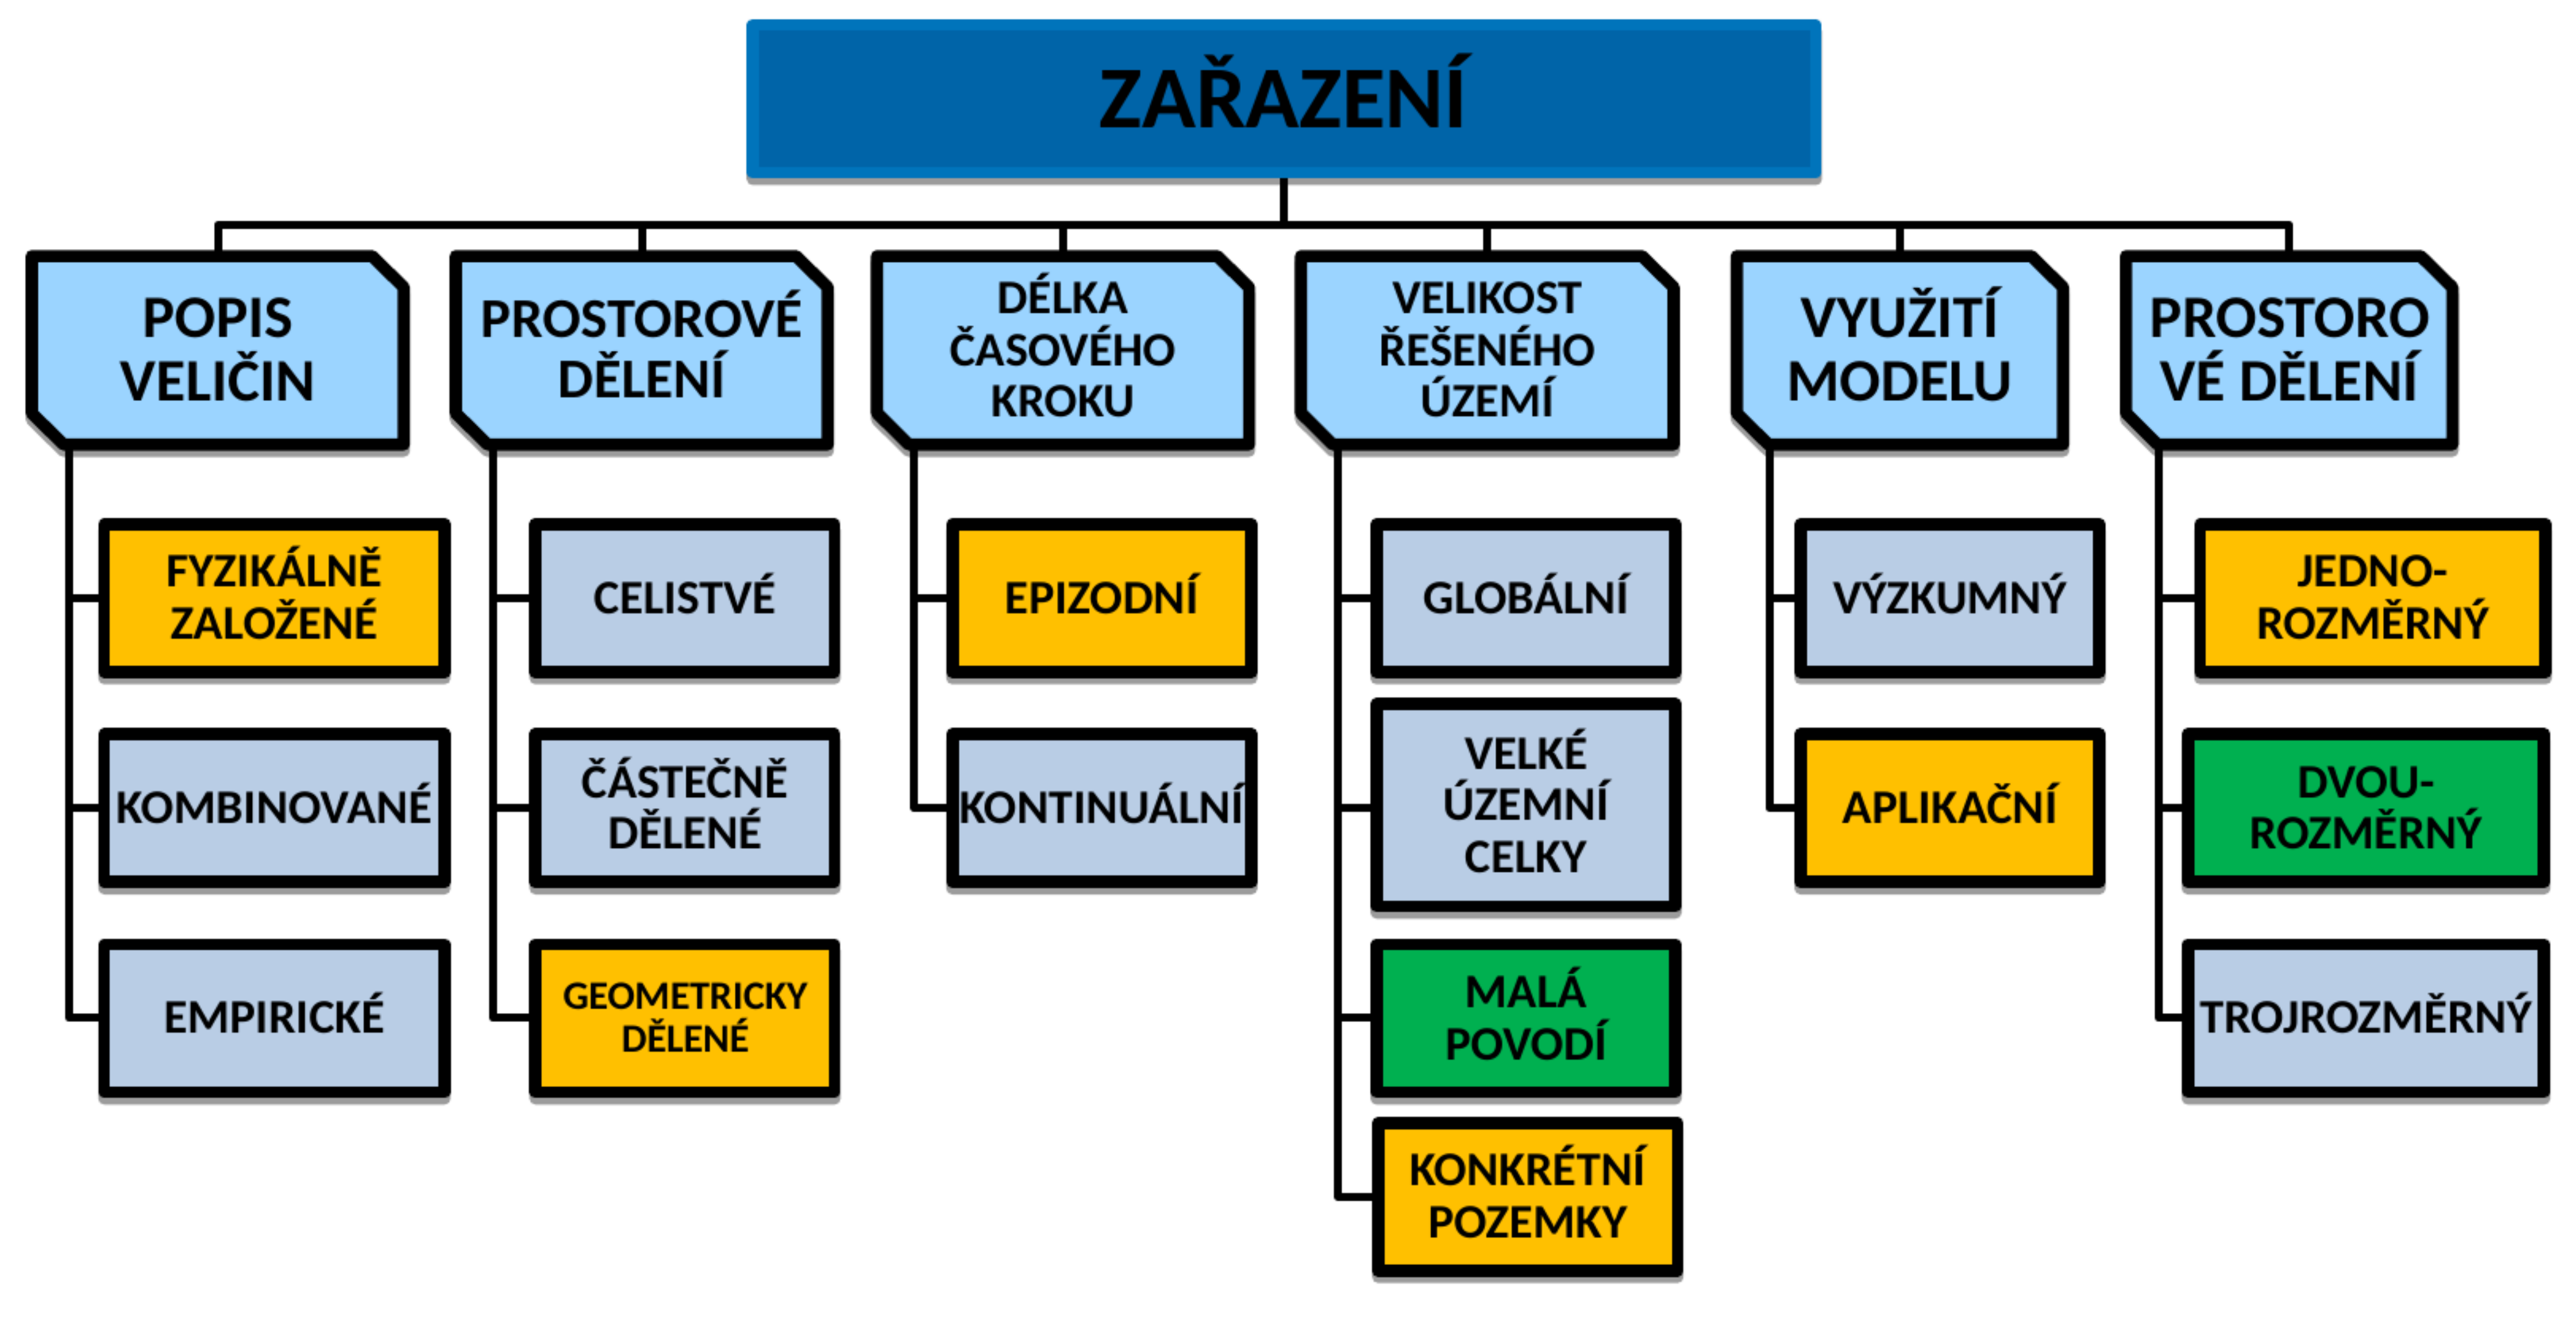
\includegraphics[width=\textwidth]{obr/vyuziti.png}
    \end{frame}

    \begin{frame}{SMODERP}
        Součást několika předpisů\\[1em]
        \begin{itemize}
            \item DOS T 3.17 - Protierozní ochrana, Váška, J., Informační centrum ČKAIT, Praha, 2000
            \item ČSN 75 4500 -  Protierozní ochrana zemědělské půdy, Český normalizační institut, 1996
            \item Janeček M., Ochrana zemědělské půdy před erozí - metodika, např. 2007, 2012
            \item Metodiky TPEO, Kadlec (2014), Dostál (2014)
            \item Kavka P., - Krátkodobé srážky pro hydrologické modelování a navrhování drobných vodohospodářských staveb v krajině, 2018
        \end{itemize}
    \end{frame}


    \section{Procesy - Parametry}
\begin{frame}{SMODERP}
\begin{itemize}\itemsep=1em
        \item Srážka
        \item Infiltrace 
            \begin{itemize}
                \item Philipova infiltrace
            \end{itemize}
        \item Povrchová retence
        \item Vliv vegetace
            \begin{itemize}
                \item intercepce, poměrná plocha listová
            \end{itemize}
        \item Povrchový odtok
            \begin{itemize}
                \item plošný, soustředěný odtok
                \item parametry power law 
                \item drsnost pro soustředěný odtok
            \end{itemize}
        \item Odtok hydrografickou sítí (Jen 2D)
            \begin{itemize}
                \item parametry úseků hydrografické sítě
            \end{itemize}
\end{itemize}
\end{frame}

    \section{Model}

    \begin{frame}{SMODERP1D}
        \begin{columns}
            \begin{column}{0.5\textwidth}
                Posouzení erozní ohroženosti 
                \begin{itemize}
                    \item návrh změny osevních postupů
                    \item umístění ochranných travních pásů
                    \item návrh pásového střídání plodin
                \end{itemize}\vspace{1em}
                Výpočet charakteristik protierozních opatření
                \begin{itemize}
                    \item záchytné a odváděcí prvky
                    \item zasakovací prvky
                    \item prvky měnící podélný sklon
                    \item dráhy soustředěného odtoku
                    \item ochranné nádrže
                \end{itemize}\vspace{1em}
                ke stažení:
                \href{http://storm.fsv.cvut.cz/cinnost-katedry/volne-stazitelne-vysledky/smoderp/smoderp1d/?lang=cz}{storm.fsv.cvut.cz/../smoderp1d/}
            \end{column}
            \begin{column}{0.5\textwidth}
                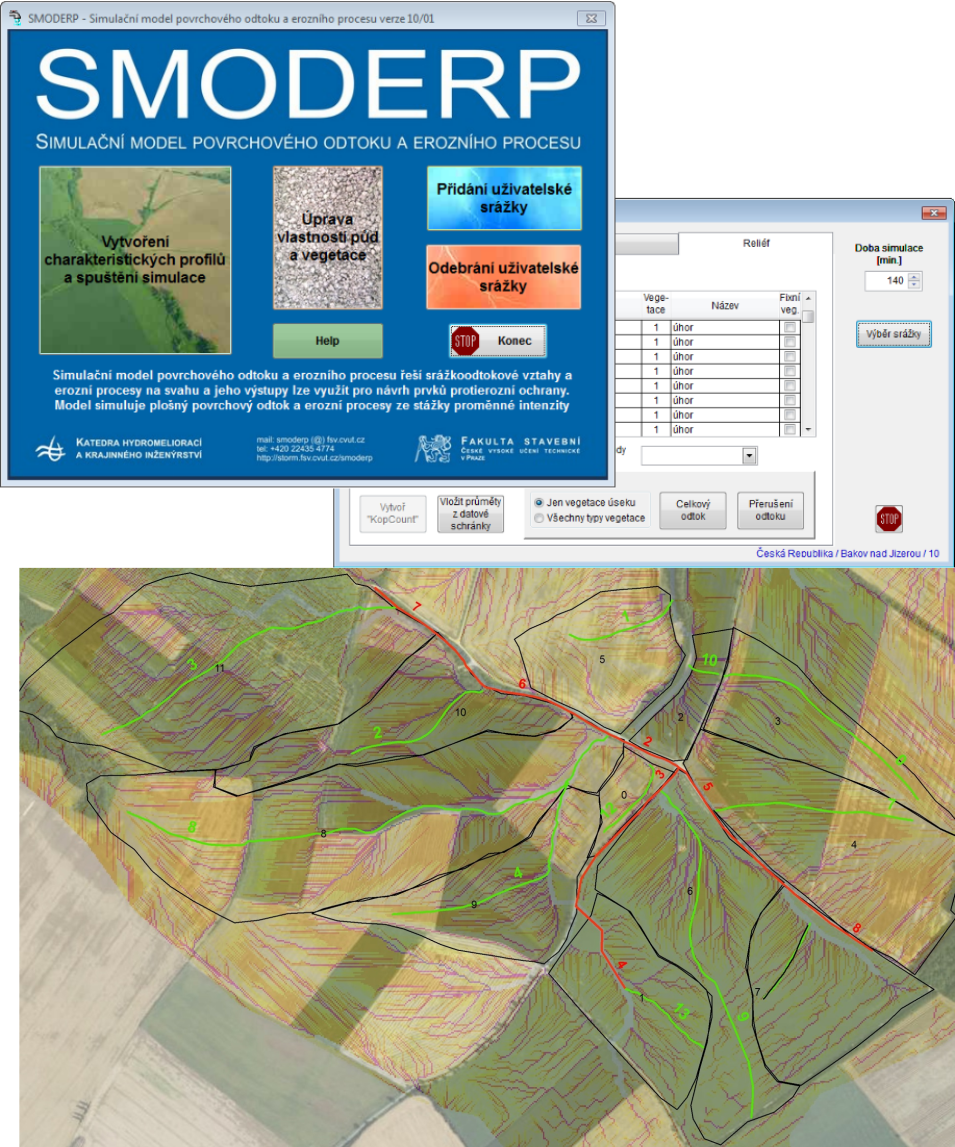
\includegraphics[width=\textwidth]{obr/smode1d.png}
            \end{column}
        \end{columns}
    \end{frame}

    \begin{frame}{SMODERP2D}
    \begin{itemize}\itemsep=1em
            \item Model implementovaný v jazyce {\tt python}
            \item Příprava dat pomocí ArcPy
            \item Oddělený výpočet plošného odtoku, soustředěného odtoku v rýhách
                \begin{itemize}
                    \item dynamické zvětšování rýhy po překročení hraniční hodnoty
                \end{itemize}
            \item Odtok hydrografickou sítí
            \item Dynamický časový krok
            \item Jednosměrný odtokový algoritmus
       \end{itemize}
       \hfill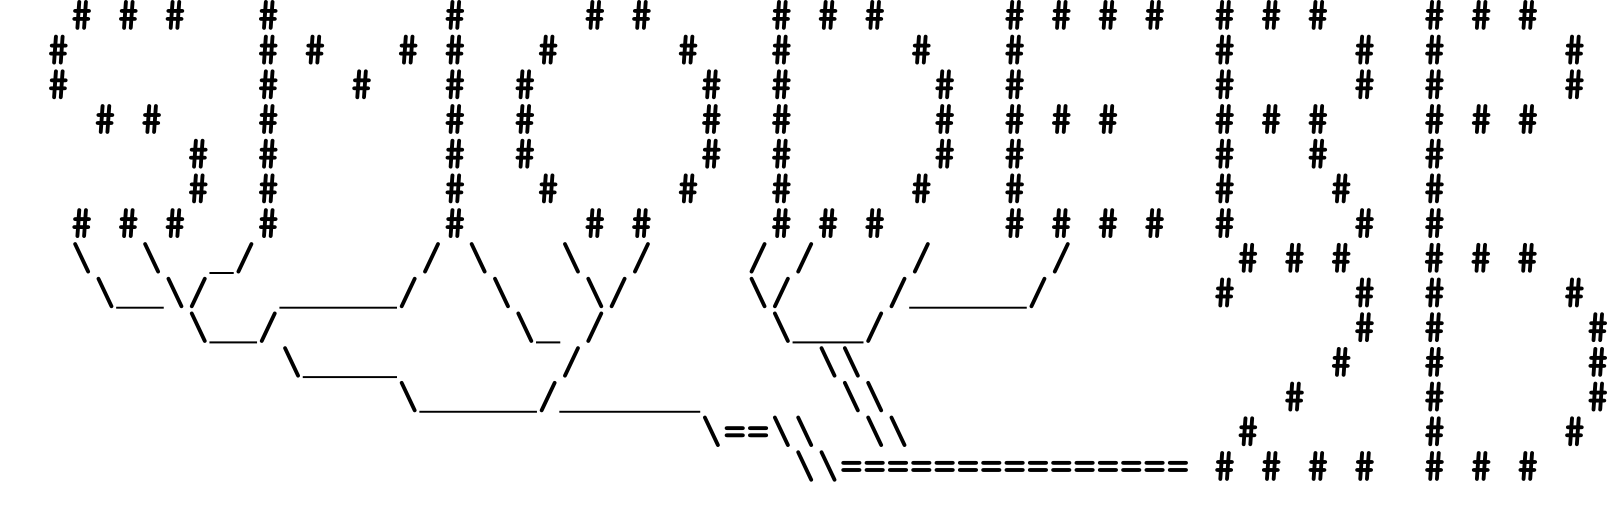
\includegraphics[height=0.175\textheight]{loga/logsmoderp.png}
    \end{frame}

        \subsection{Použití}

        \begin{frame}
            ArcGIS toolbox:\vspace{-1em}
            \begin{figure}[t!]
            \centering
            \begin{minipage}[t]{.4\textwidth}
              \centering
              \vspace{0pt}
                \begin{figure}
                    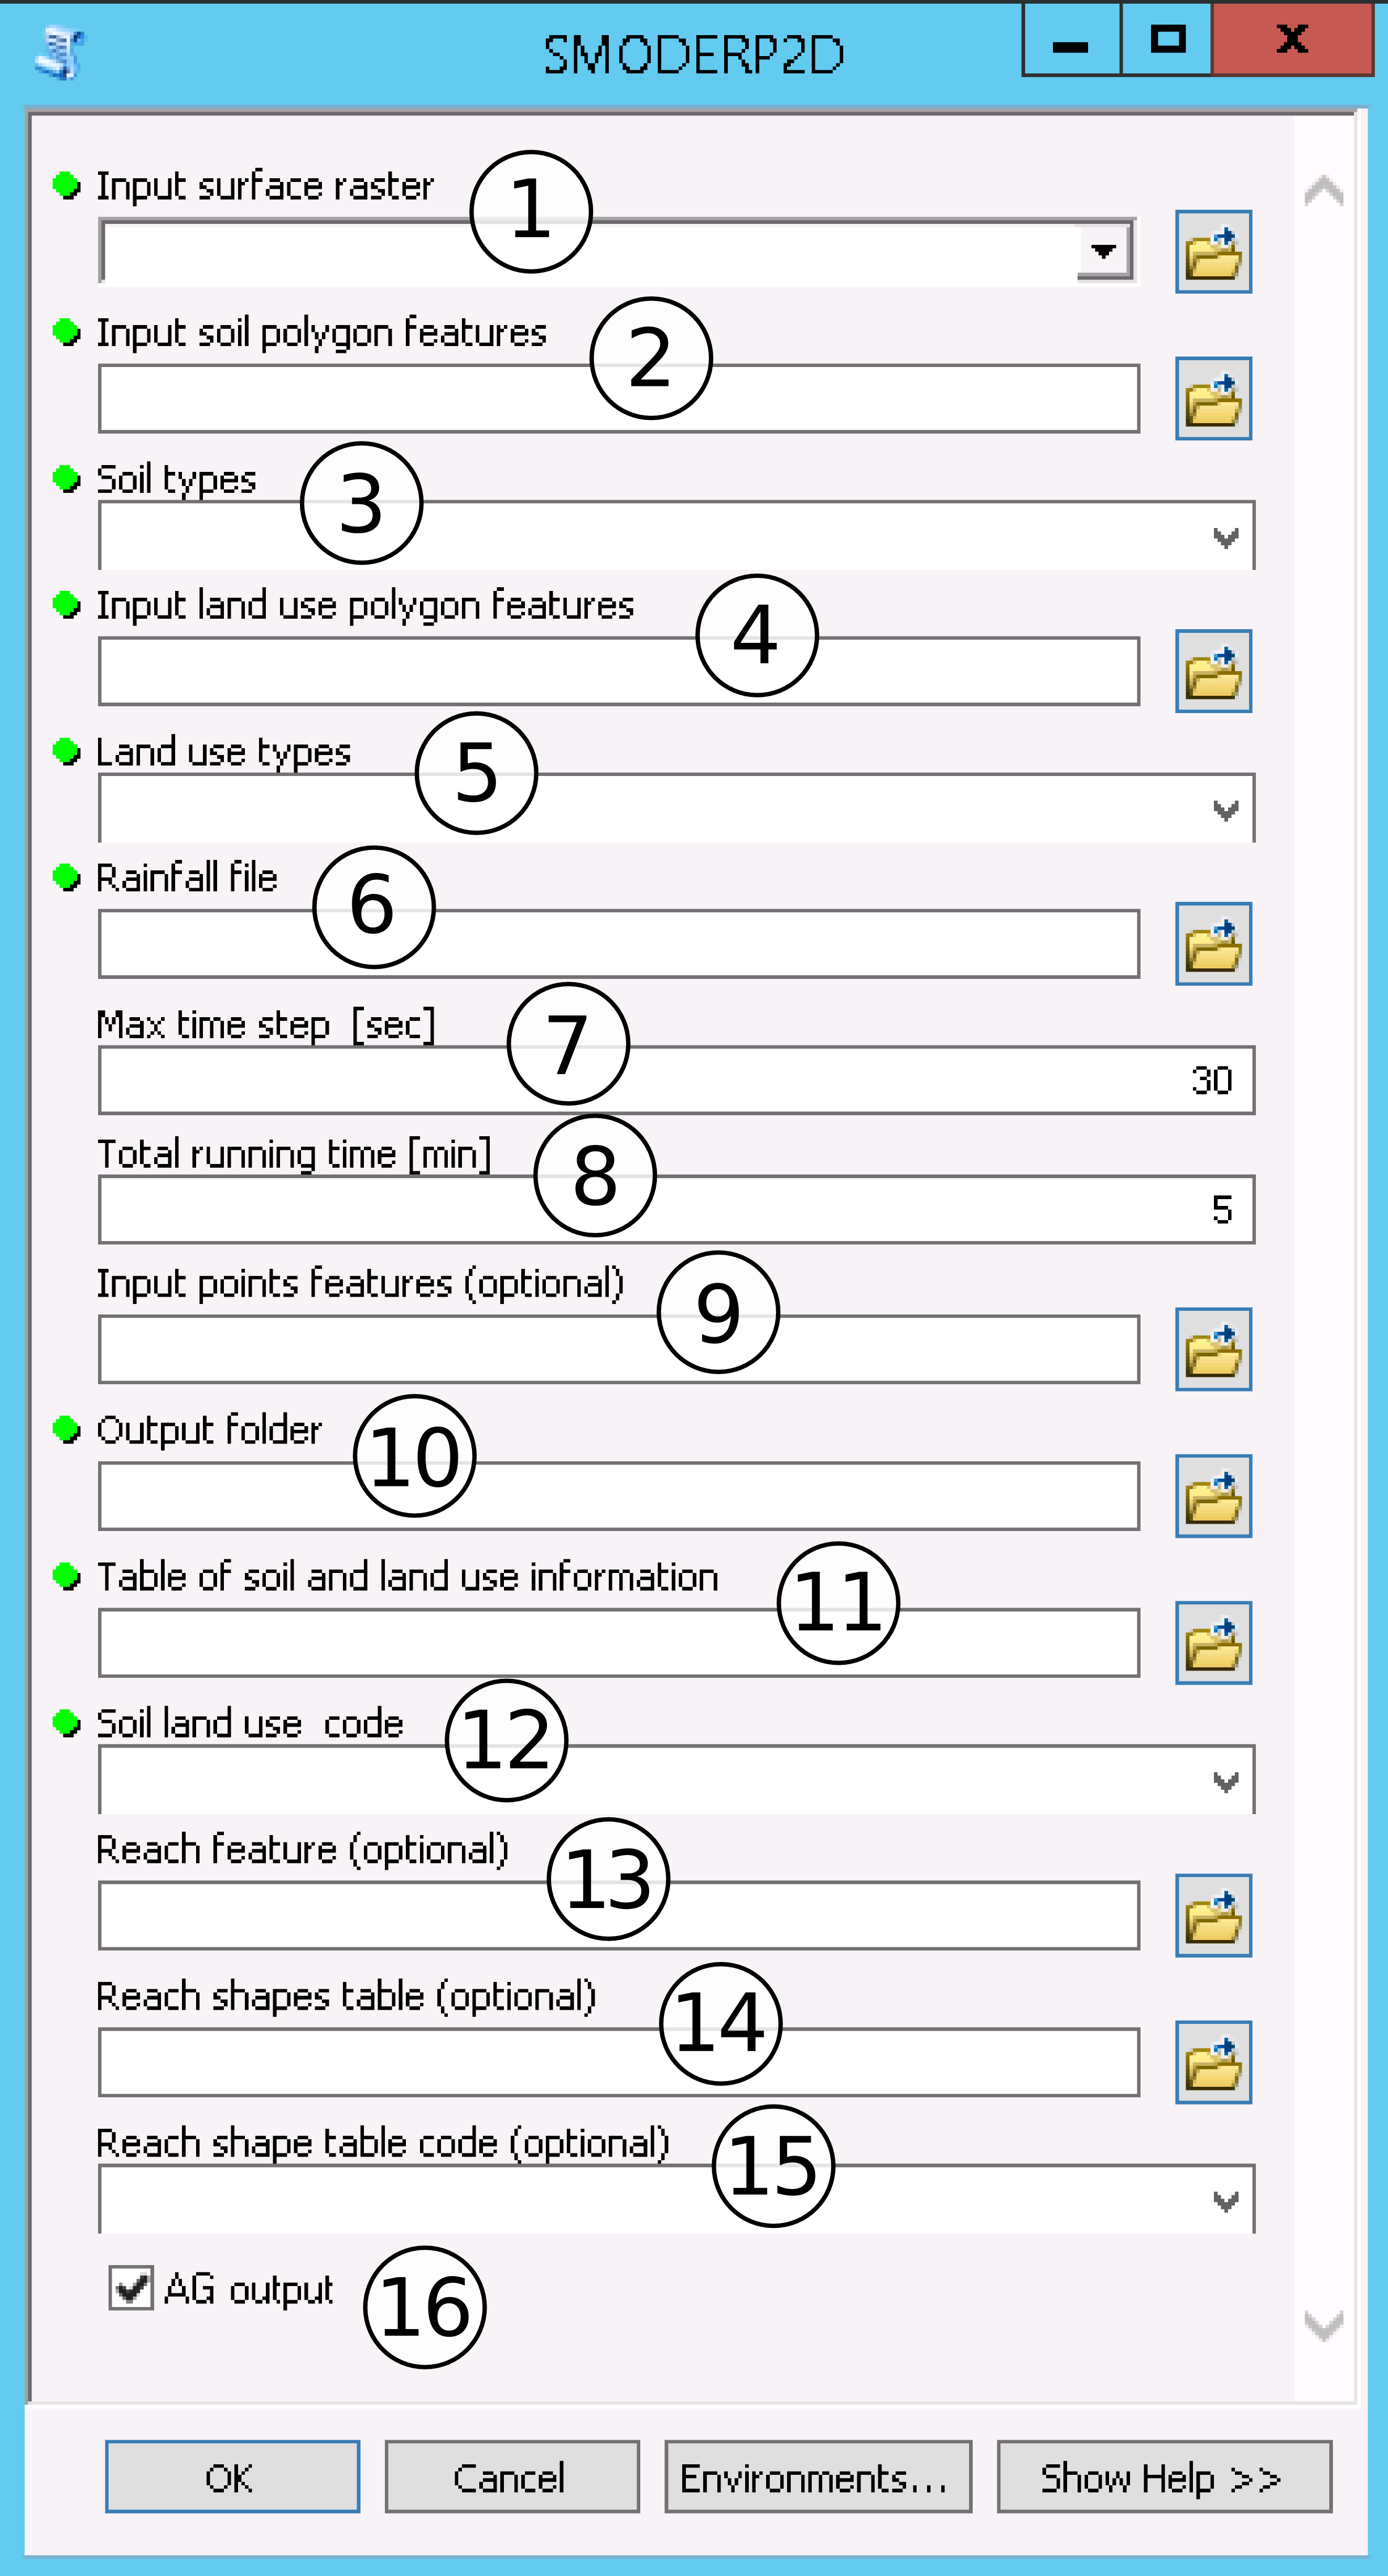
\includegraphics[width=\textwidth]{obr/toolboxpopis4.png}
                \end{figure}
            \end{minipage}\hfill
            \begin{minipage}[t]{.5\textwidth}
              \centering
              \vspace{0pt}
              {\tiny\sffamily
              \begin{tabular}{lp{.5\textwidth}l}
                             & Popis                                       & ArcGIS typ dat     \\
                \hline
            \circled{1}  & Cesta k digitálnímu modlu terénu            &  {\tt Raster layer} \\
            \circled{2}  & Cesta k vektorové vrstvě rozložení typu půd &  {\tt Shapefile} \\
            \circled{3}  & Název pole s id typů půd &  {\tt Field} \\
            \circled{4}  & Cesta k vektorové vrstvě využití území &  {\tt Shapefile} \\
            \circled{5}  & Název pole s id využití území &  {\tt Field} \\
            \circled{6}  & Cesta k souboru se srážkovými daty &  {\tt Text file} \\
            \circled{7}  & Maximální časový krok &  {\tt Double} \\
            \circled{8}  & Konečný čas výpočtu &  {\tt Double} \\
            \circled{9}  & Vrstva bodů pro výpis hydrogramů &  {\tt Shapefile} \\
            \circled{10} & Výstupní adresář &  {\tt Folder} \\
            \circled{11} & Tabulka s parametry modelu &  {\tt Table} \\
            \circled{12} & Označení pole v tabulce \circled{11} &  {\tt Field} \\
            \circled{13} & Cesta k vrstvě linií hydrografické sítě &  {\tt Feature Class} \\
            \circled{14} & Cesta k tabulce s geometrií úseků hydrografické sítě &  {\tt Table} \\
            \circled{15} & Název společného pole pro spojení \circled{13} a \circled{14} &  {\tt Field} \\
            \circled{16} & Volba formy výstupních souborů &  {\tt Boolean} \\
              \end{tabular}
              }
            \end{minipage}
            %\caption{ArcGIS {\tt toolbox} a vysvětlenými parametry}
            \label{fig:toolbox}
          \end{figure}

        \end{frame}

        \begin{frame}
            Testovací data v ArcGIS\vspace{1em}
            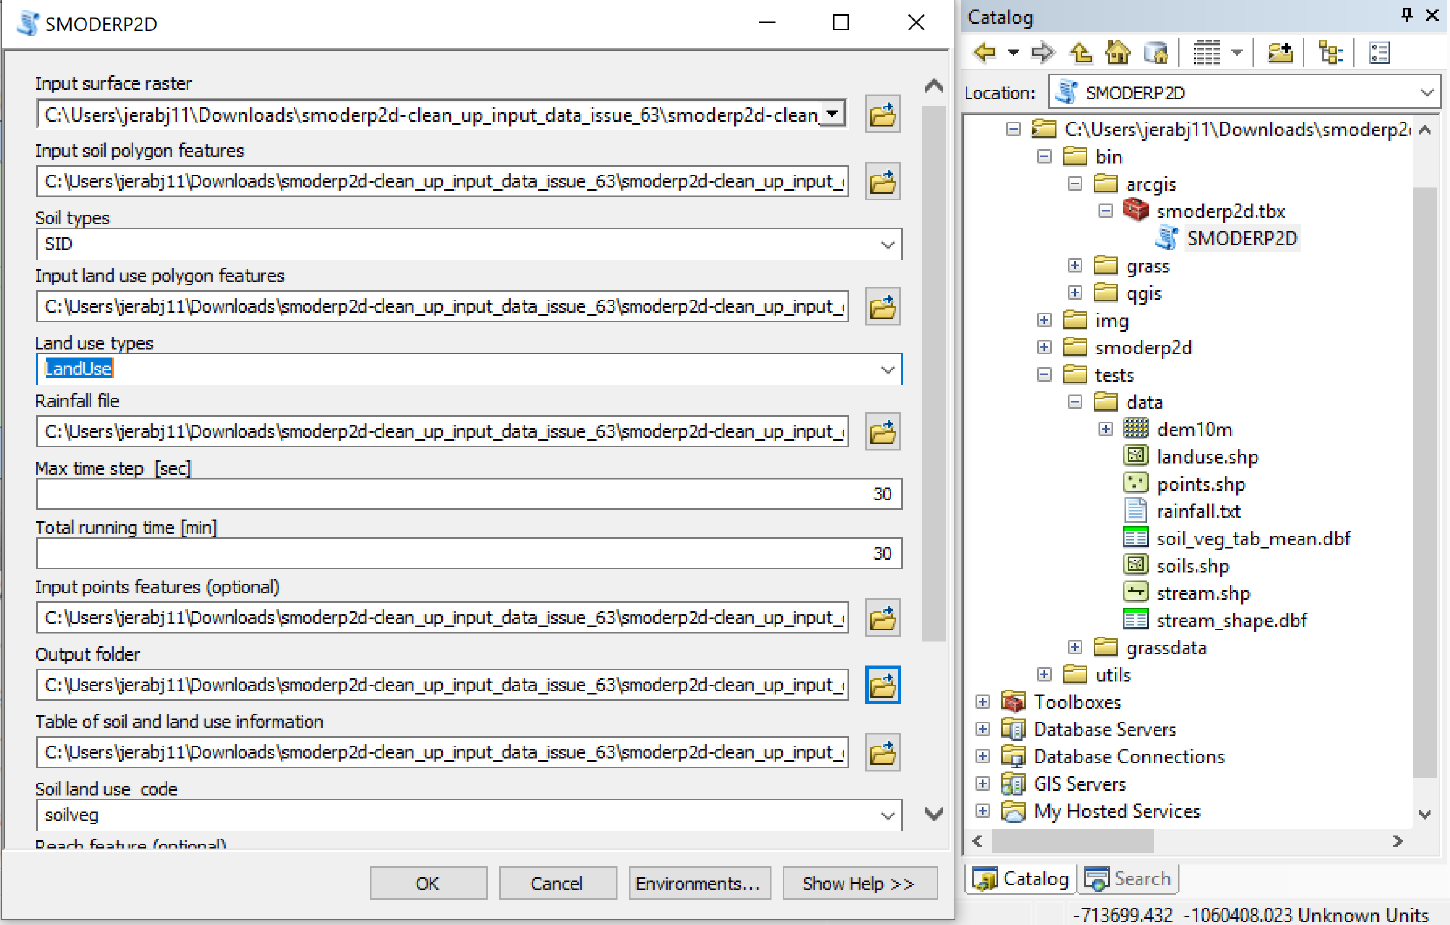
\includegraphics[width=0.95\textwidth]{obr/arcmap01.png}
        \end{frame}

        \begin{frame}\hypertarget{fig}{}
        \Wider[4em]{
            Ukázka přípravy dat v ArcGIS\vspace{1em}: půdní typ a využití území 
            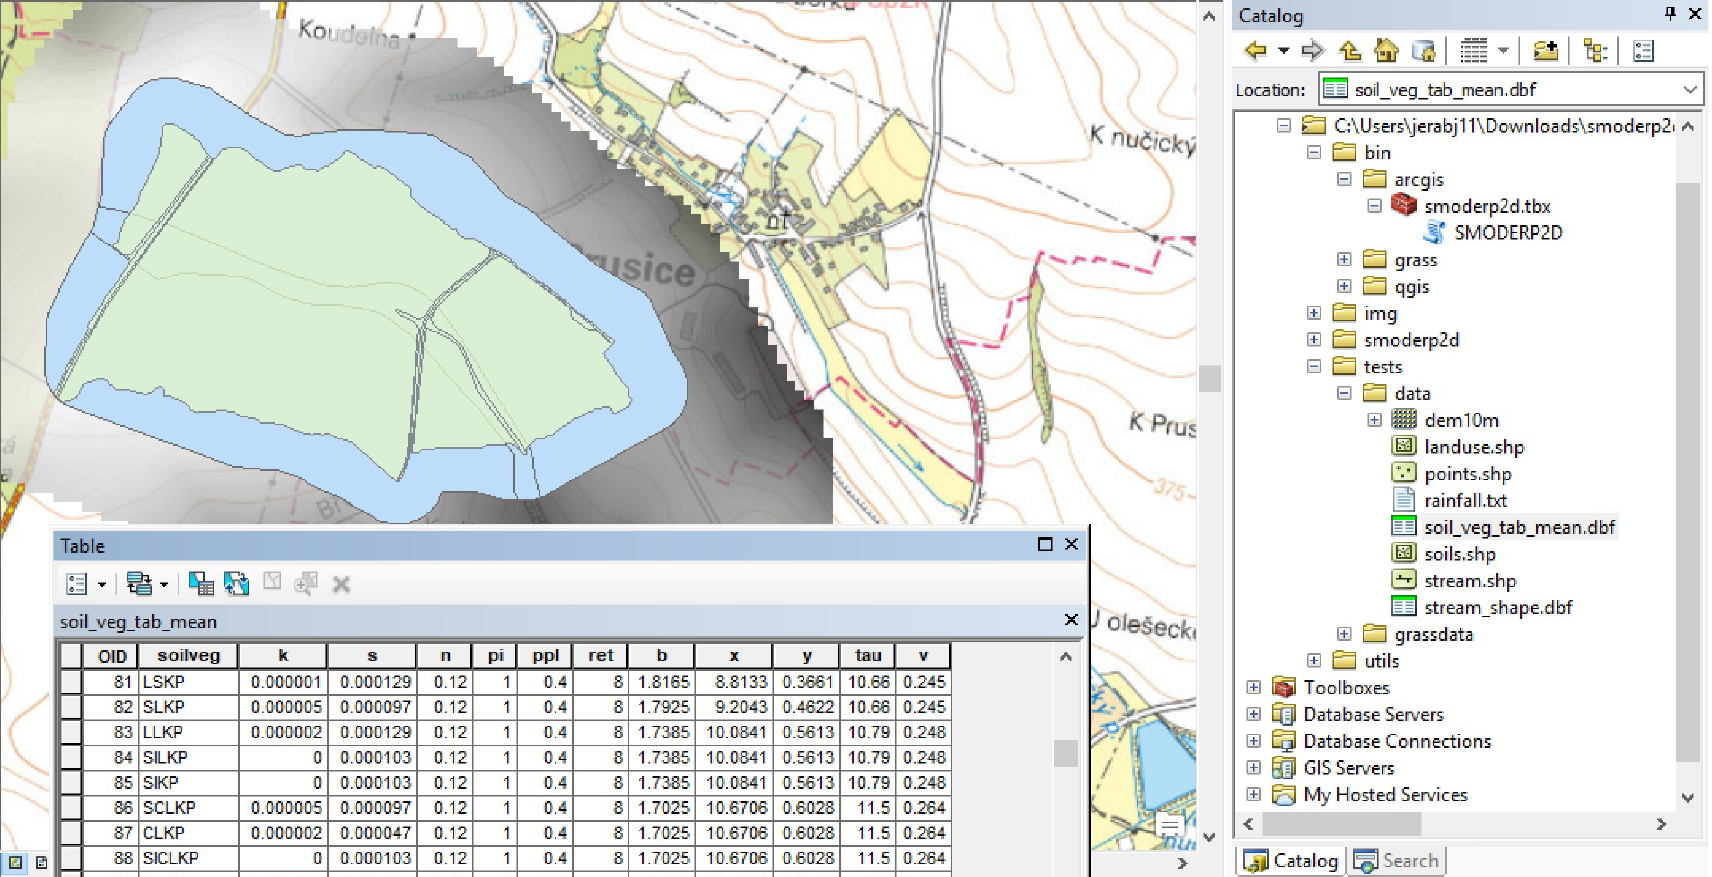
\includegraphics[width=\textwidth]{obr/arcmap02.png}
            Popis sloupečku v atributové tabulce~\ref{tab:soilveg} za konci prezentace.
        }
        \end{frame}
        \begin{frame}
        \Wider[4em]{
            Ukázka přípravy dat v ArcGIS\vspace{1em}: hydrografická síť
            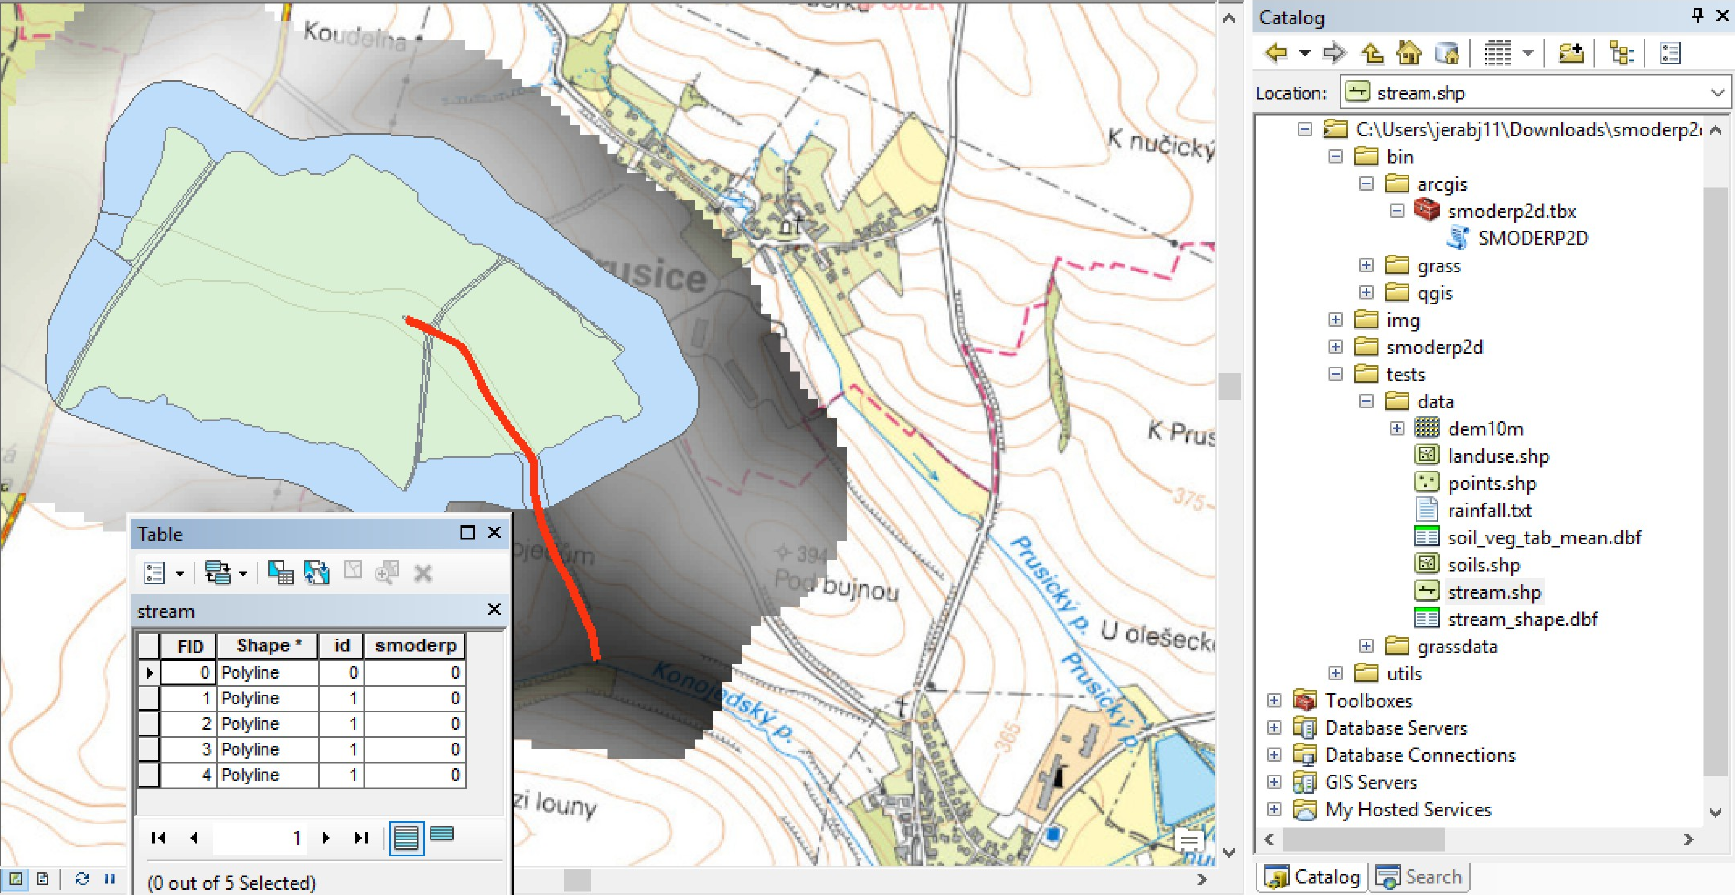
\includegraphics[width=\textwidth]{obr/arcmap03.png}
        }
        \end{frame}
        \begin{frame}
        \Wider[4em]{
            Ukázka přípravy dat v ArcGIS\vspace{1em}: parametry úseků hydrografické sítě
            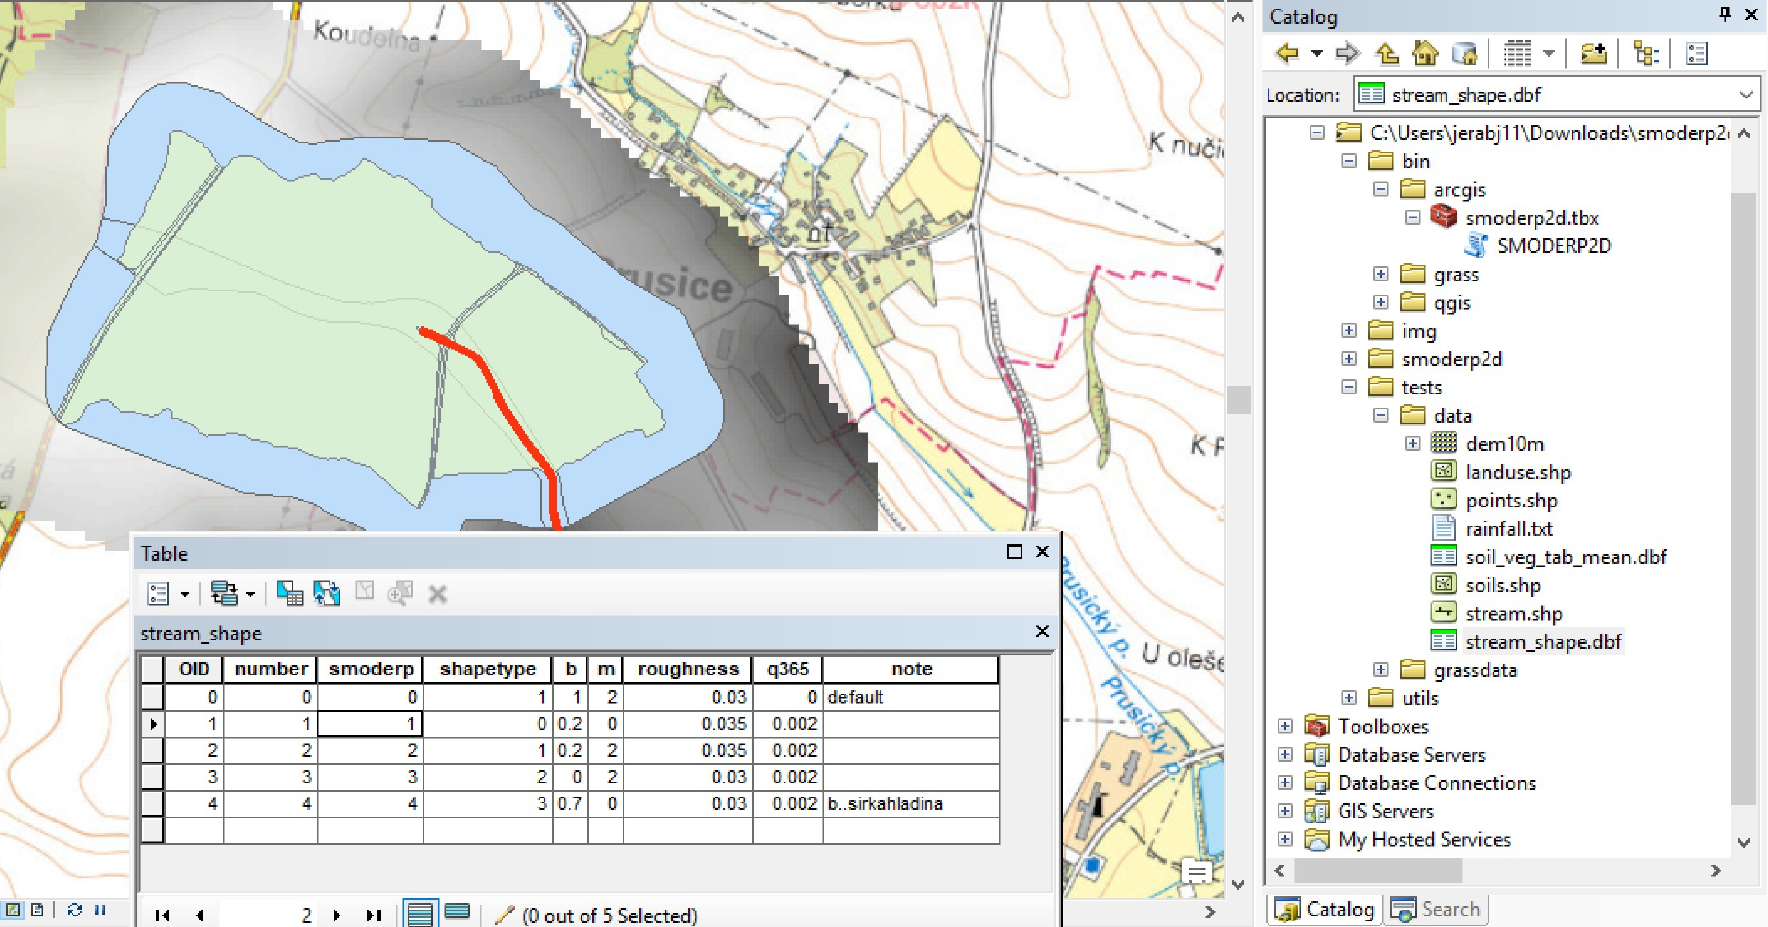
\includegraphics[width=\textwidth]{obr/arcmap04.png}
        }
        \end{frame}
        \begin{frame}
        \Wider[4em]{
            Ukázka přípravy dat v ArcGIS\vspace{1em}: body na výpis výsledků
            \begin{center}
            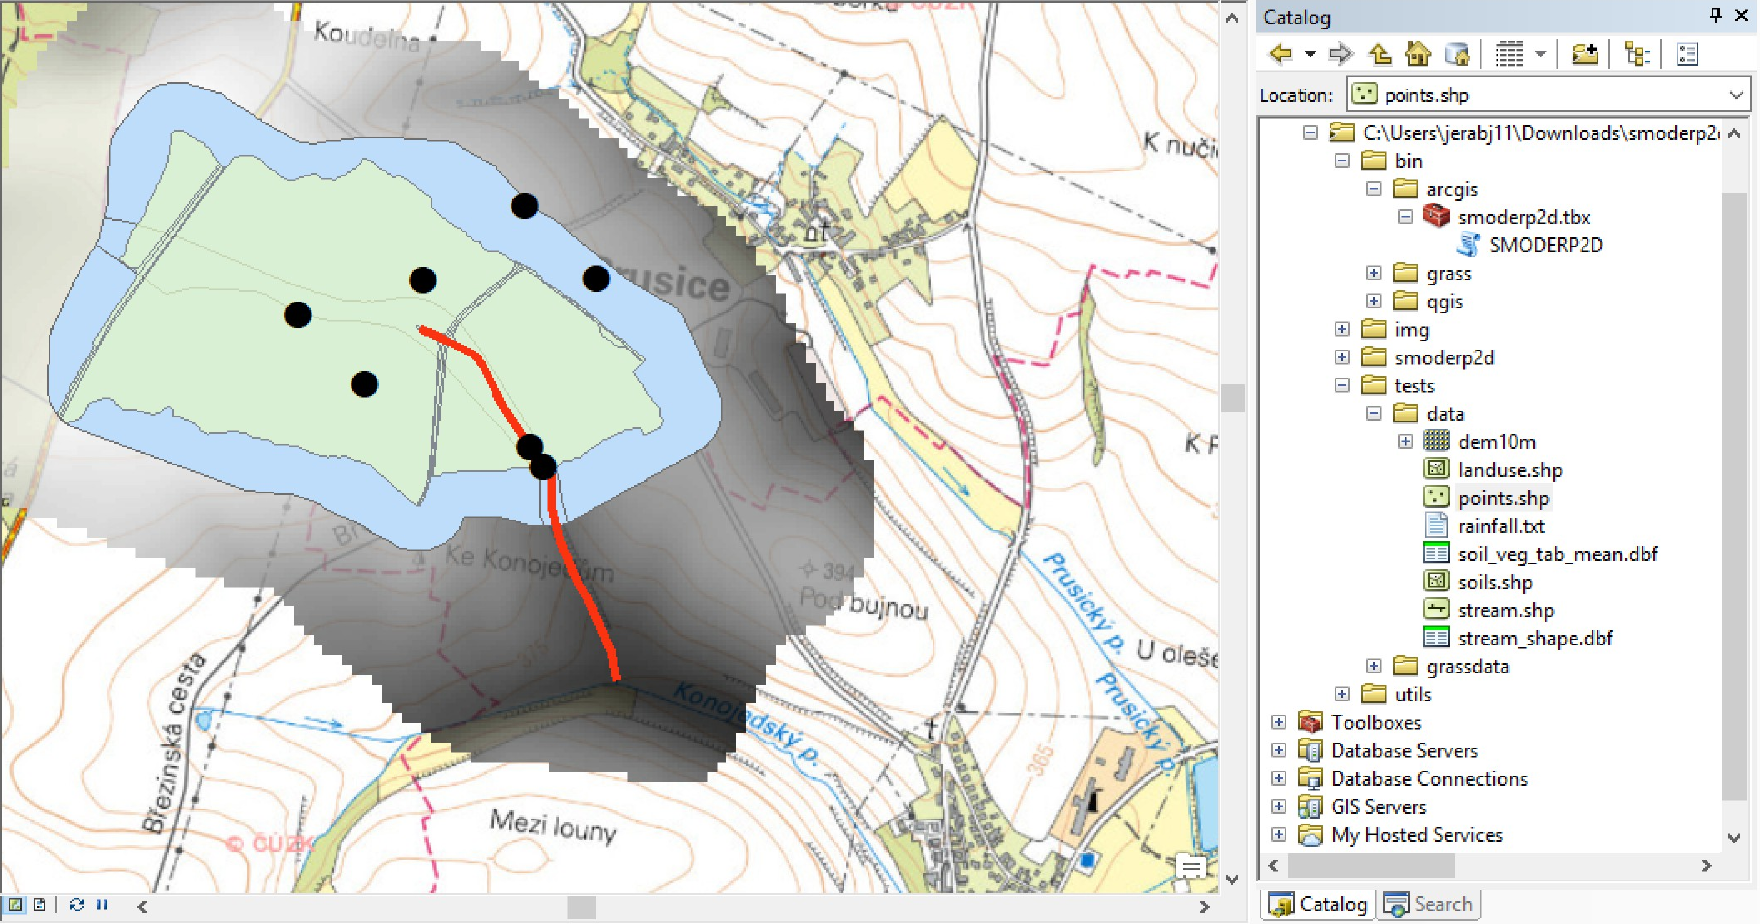
\includegraphics[width=\textwidth]{obr/arcmap05.png}
            \end{center}
        }
        \end{frame}


        \begin{frame}[plain]
            Ukázka výsledků reakce povodí na 40 minut 120 mm/hod srážky
            \begin{adjustwidth}{-3em}{-2em}
                    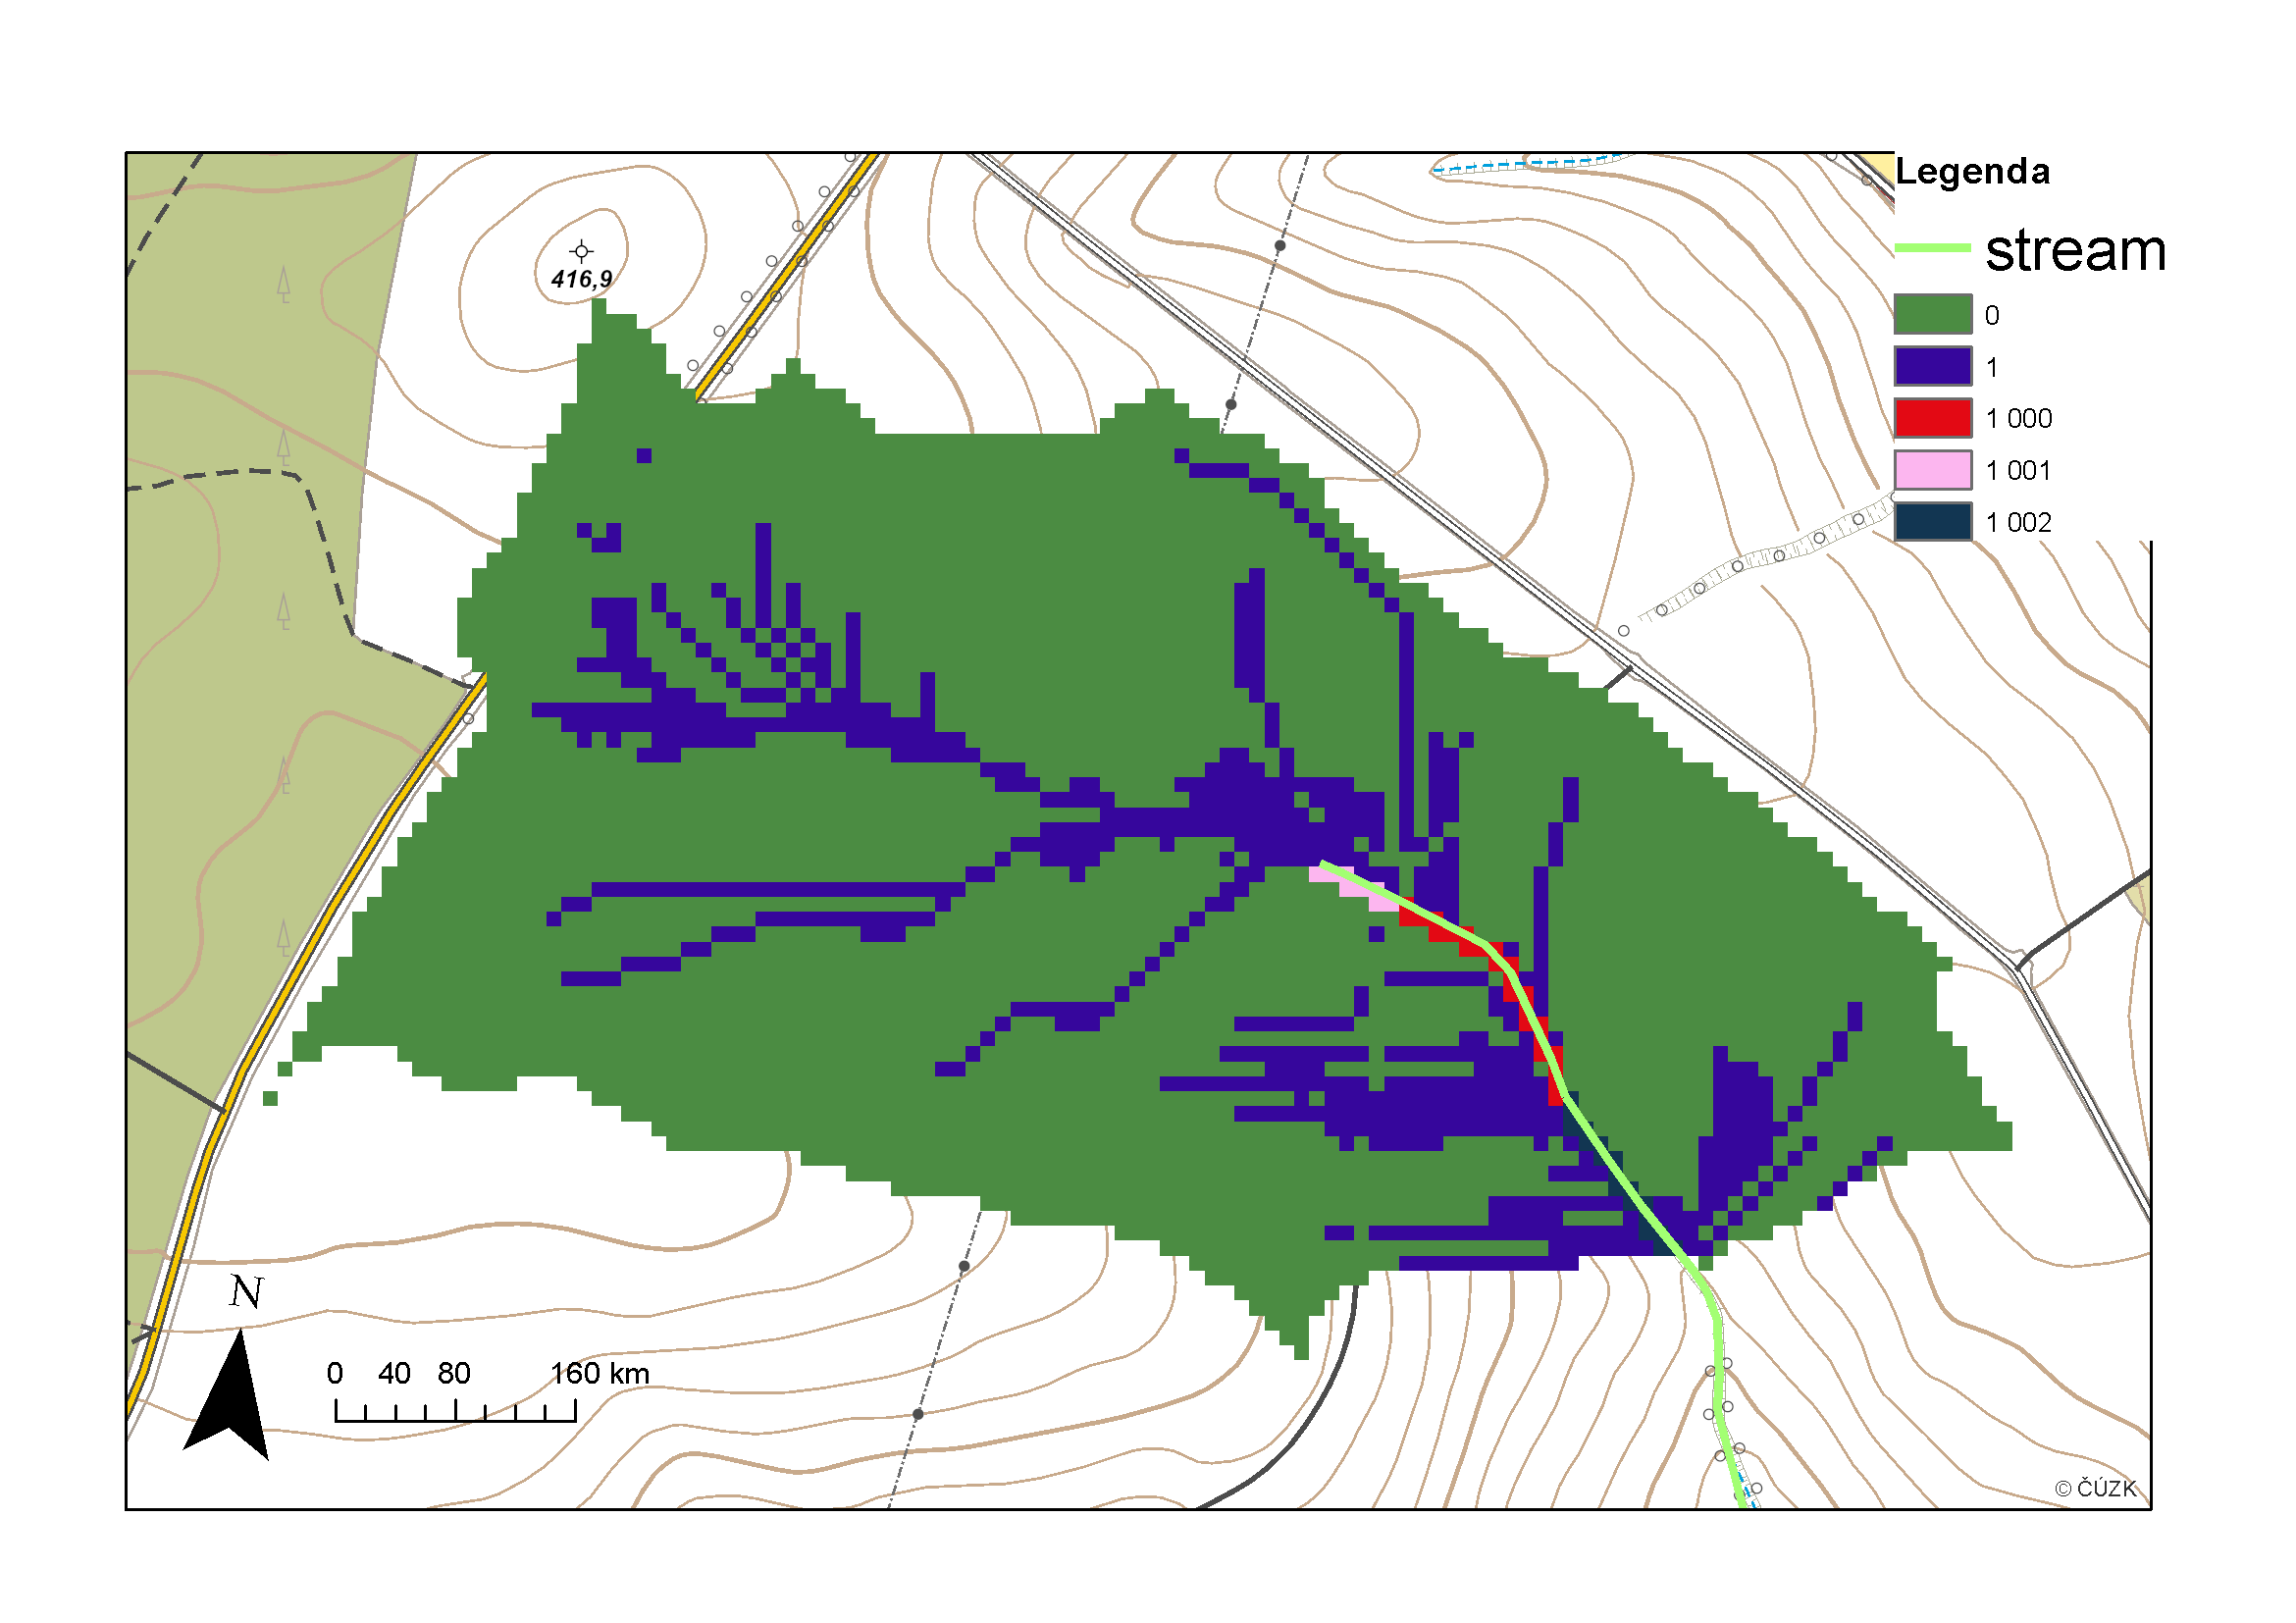
\includegraphics[width=0.55\textwidth]{obr/fstate.png}
                    %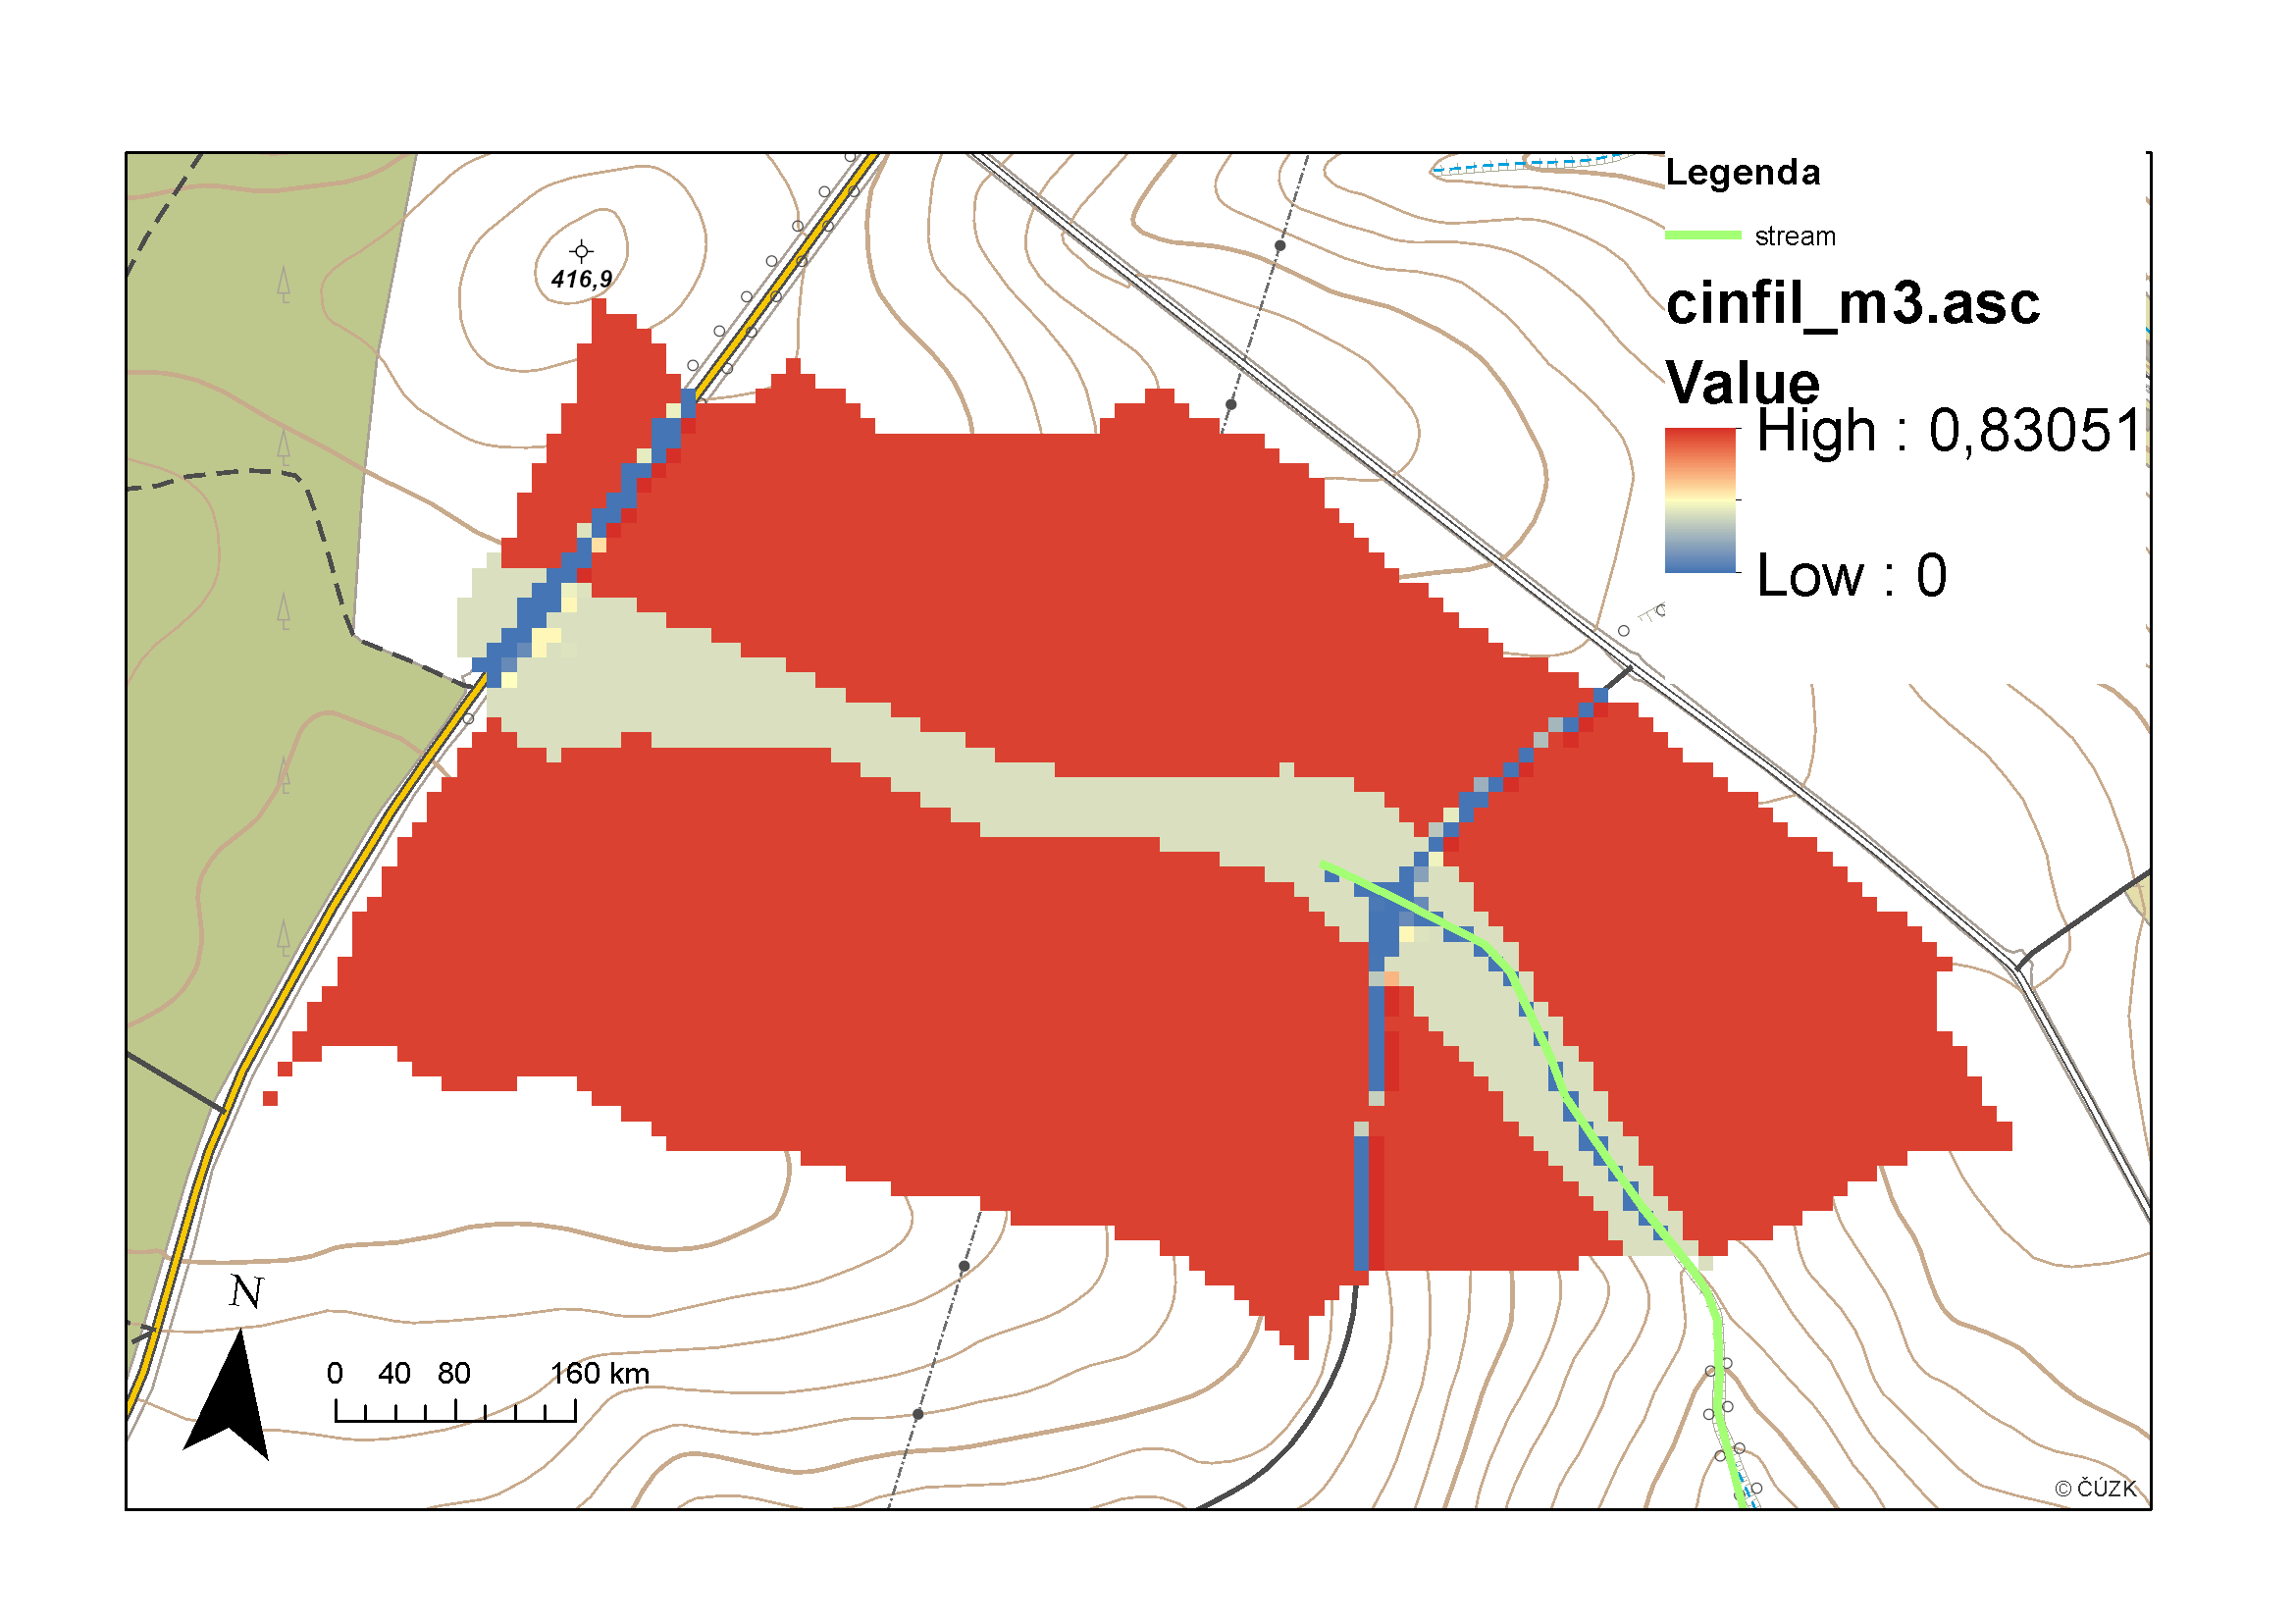
\includegraphics[width=0.55\textwidth]{obr/infiltr.png}\\
                    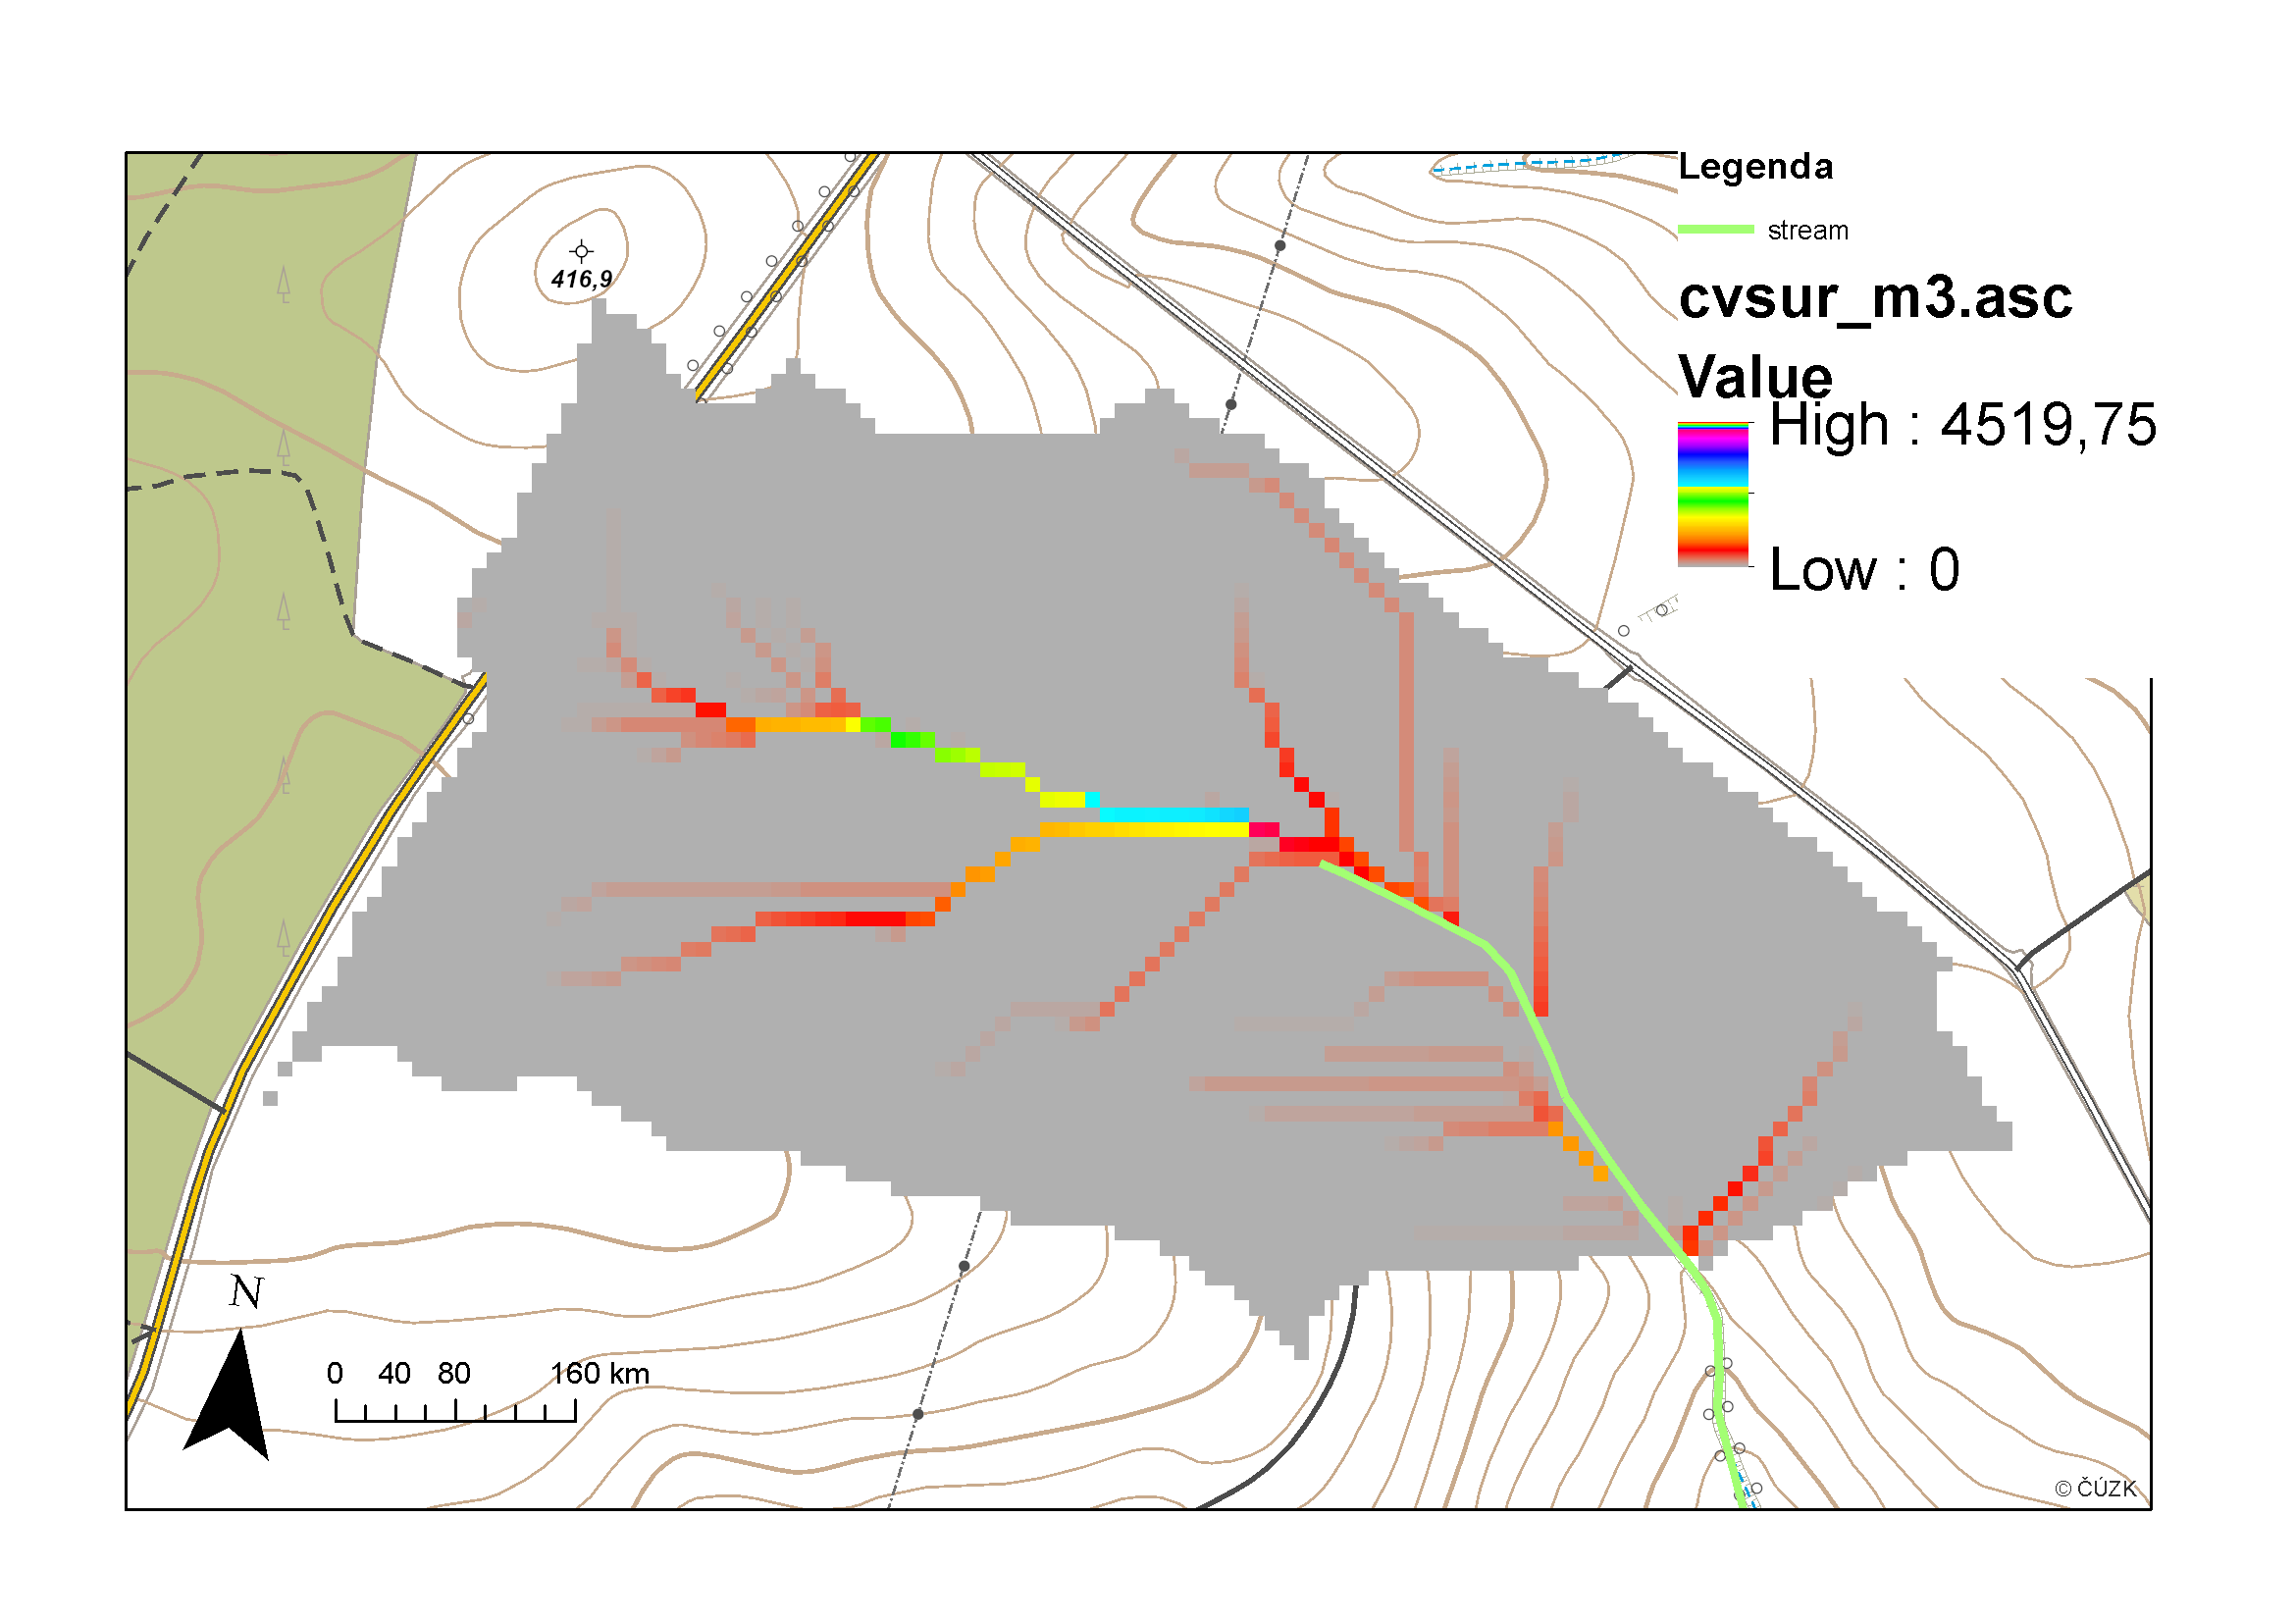
\includegraphics[width=0.55\textwidth]{obr/cvsur.png}\\
                    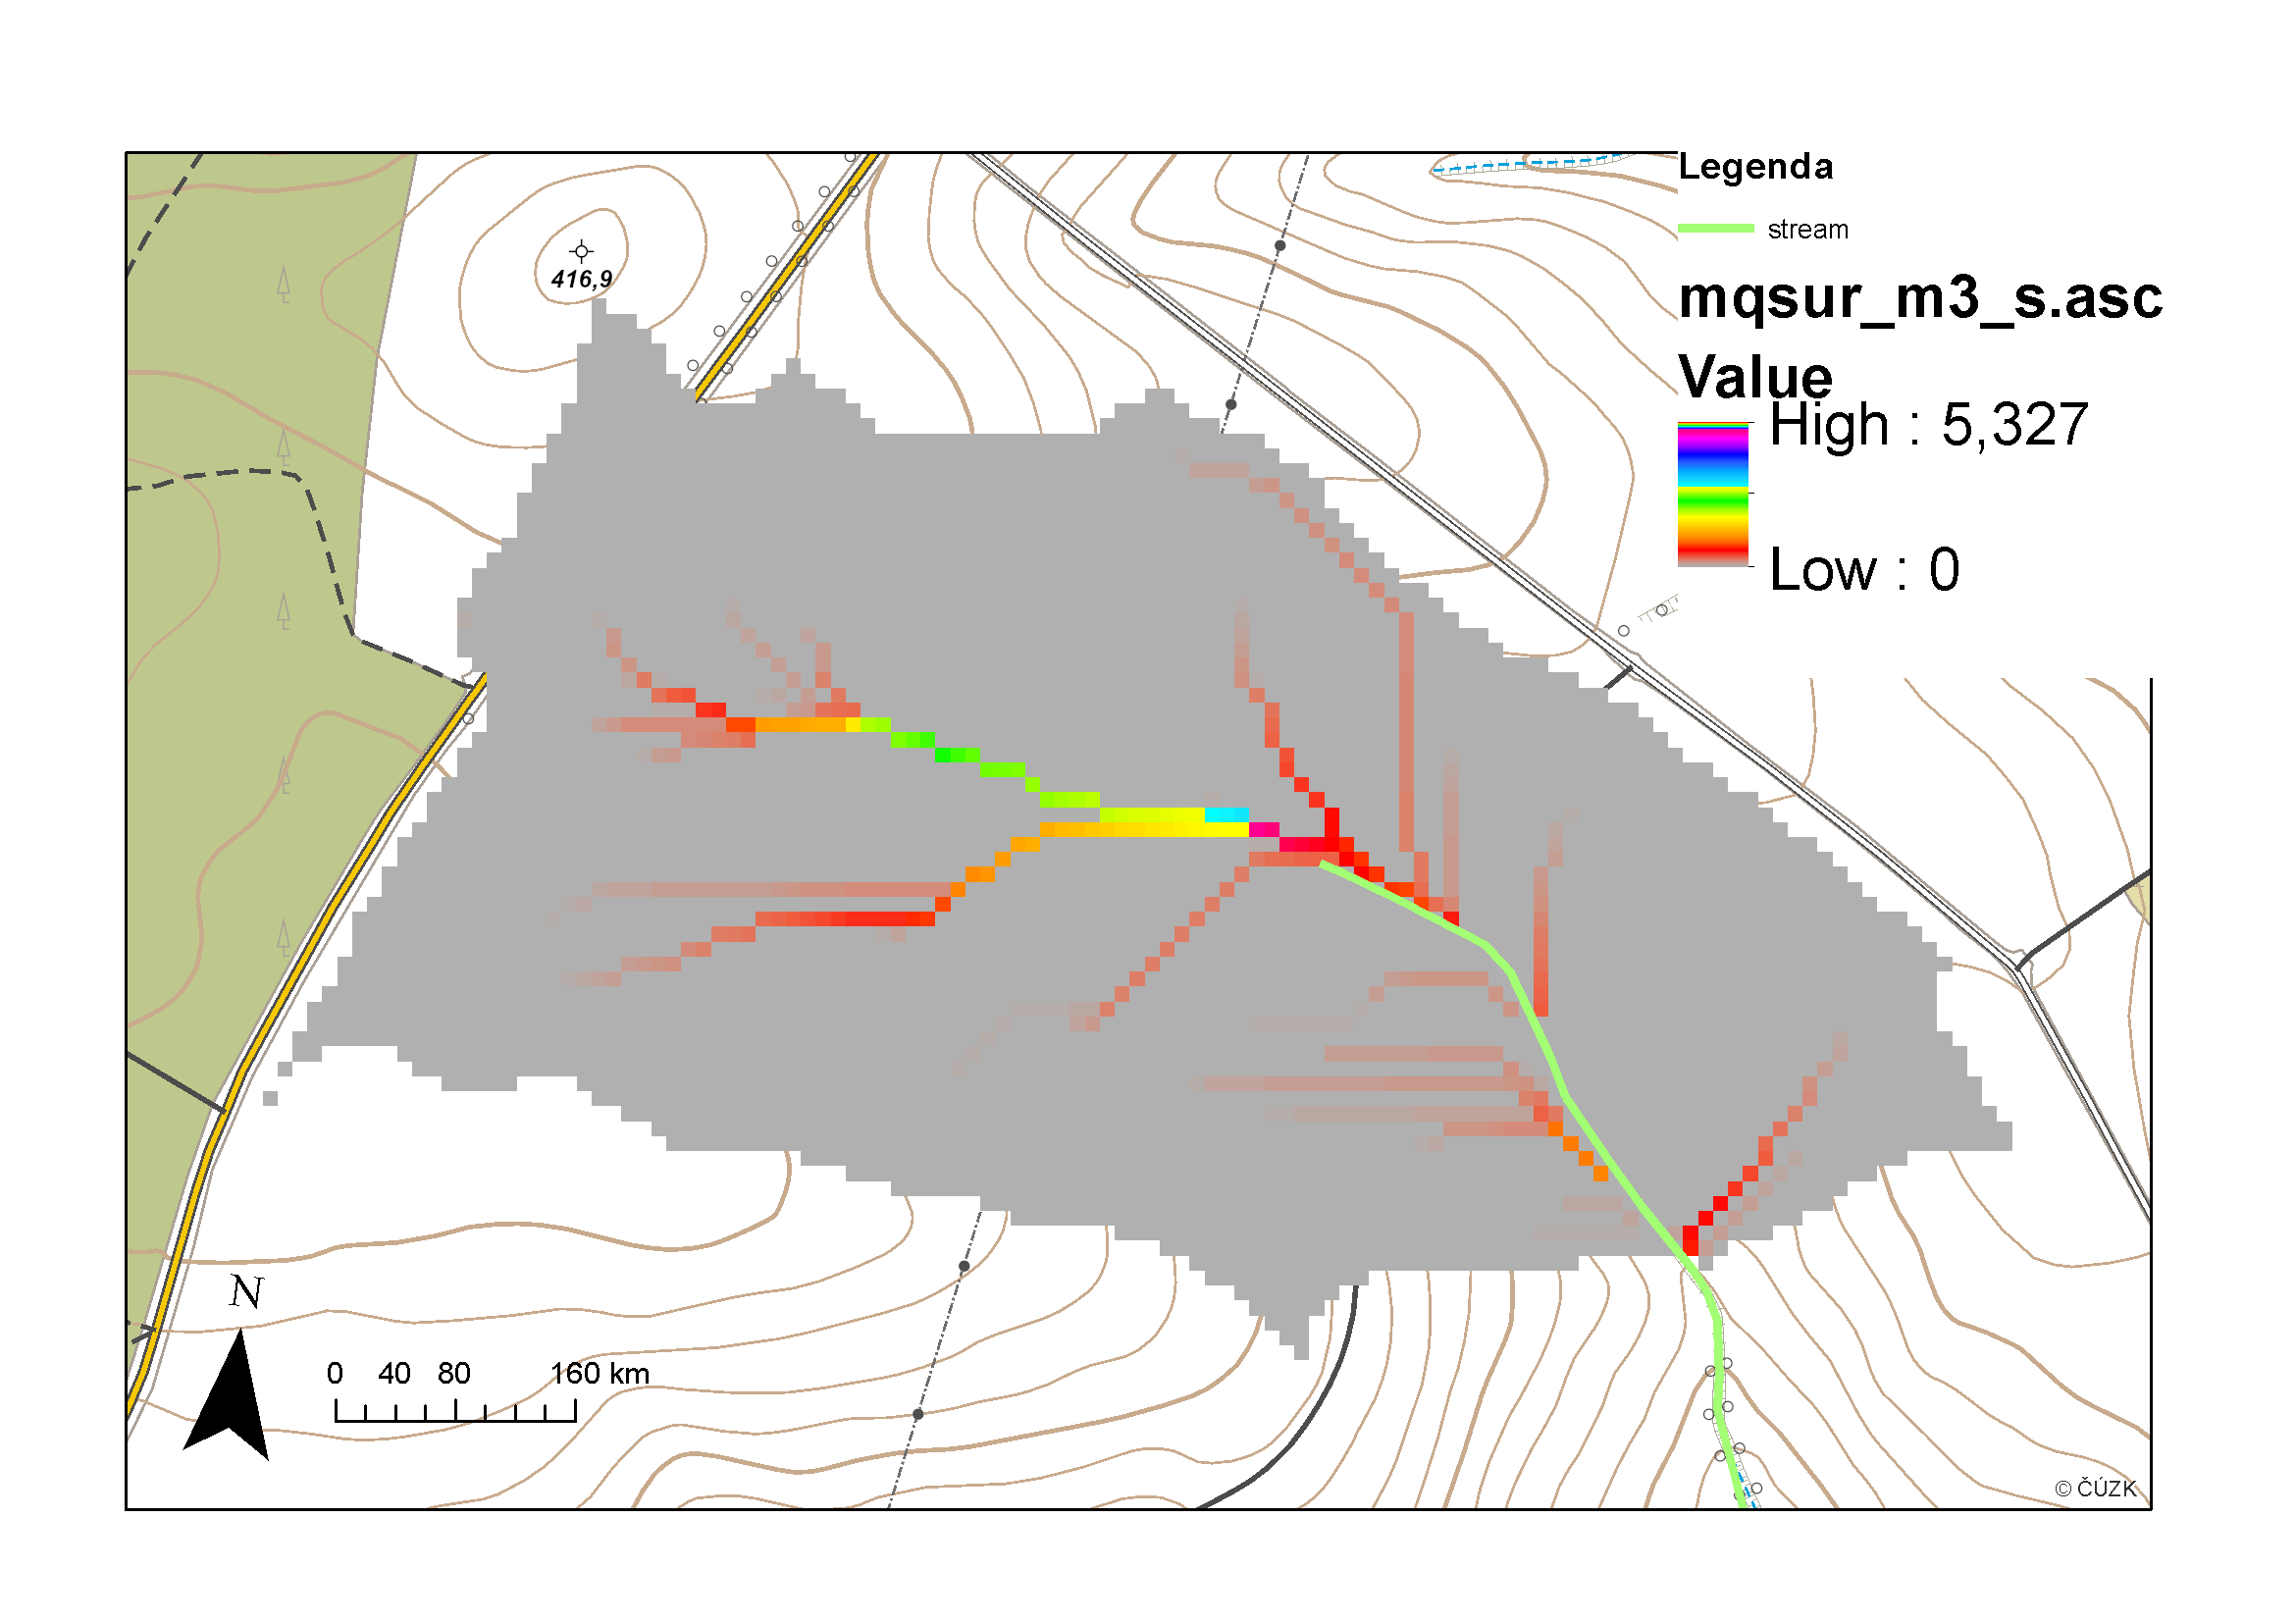
\includegraphics[width=0.55\textwidth]{obr/mqsur.png}
                    %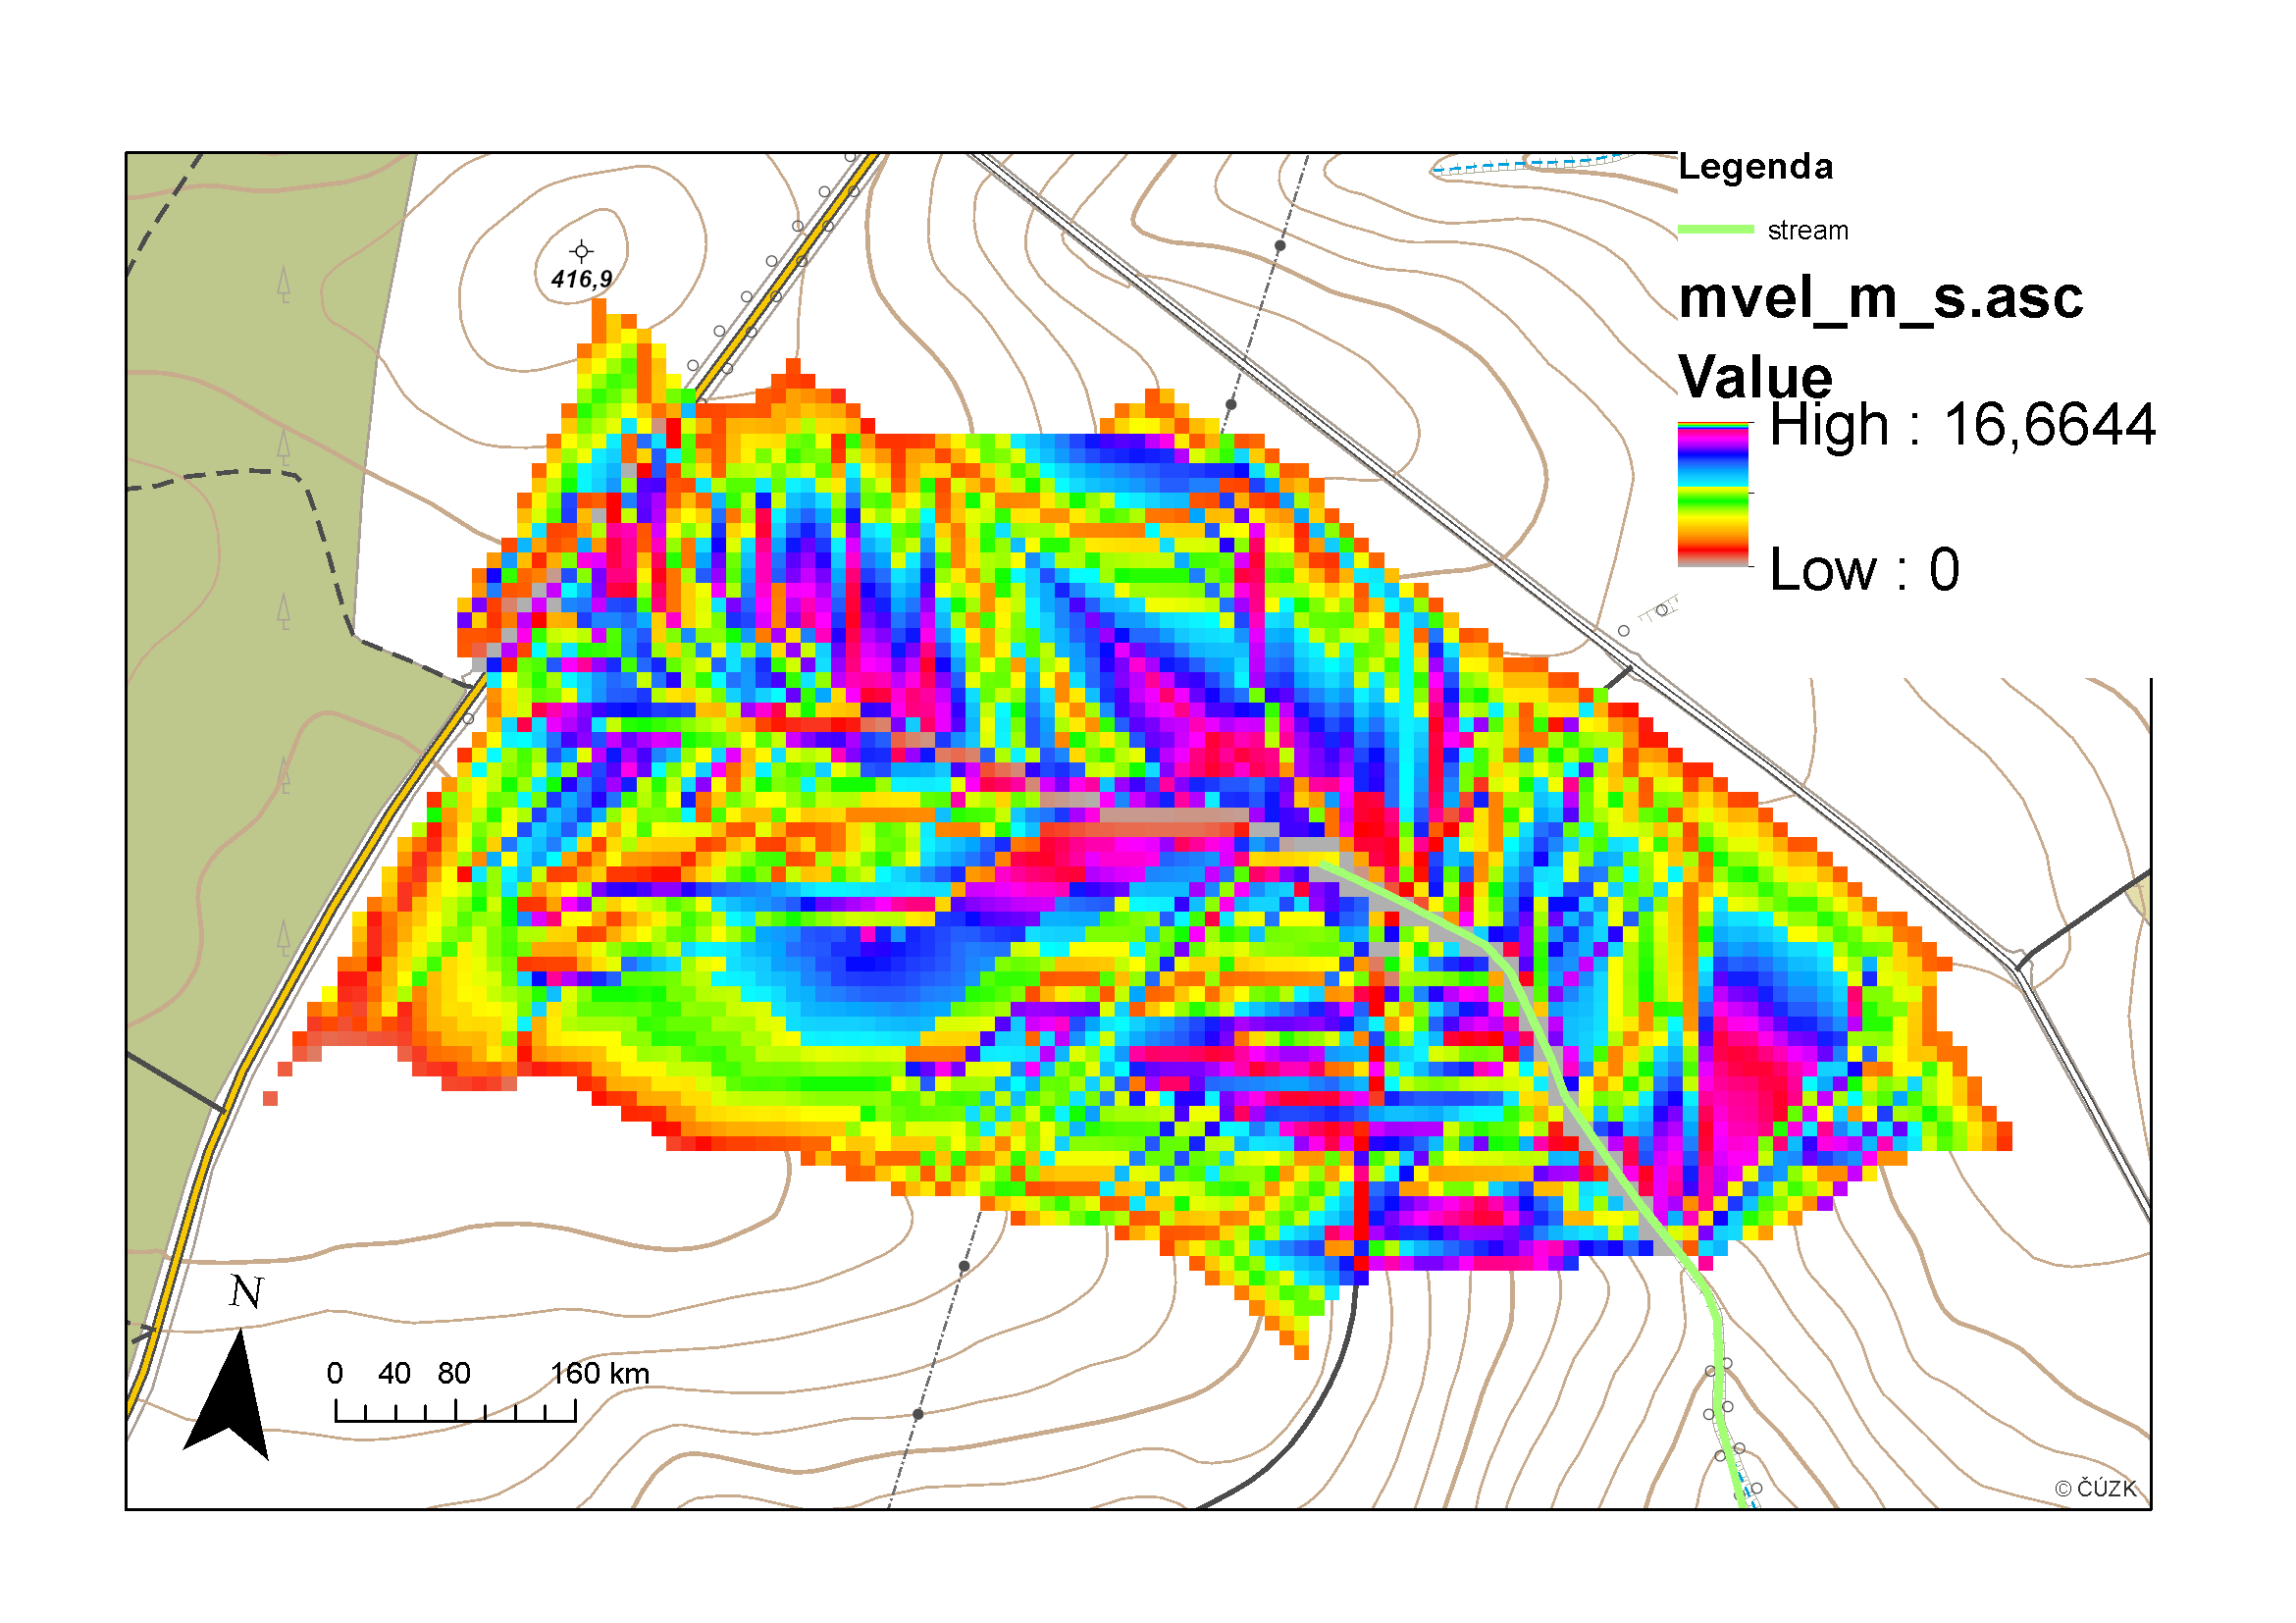
\includegraphics[width=0.55\textwidth]{obr/mvel.png}
                    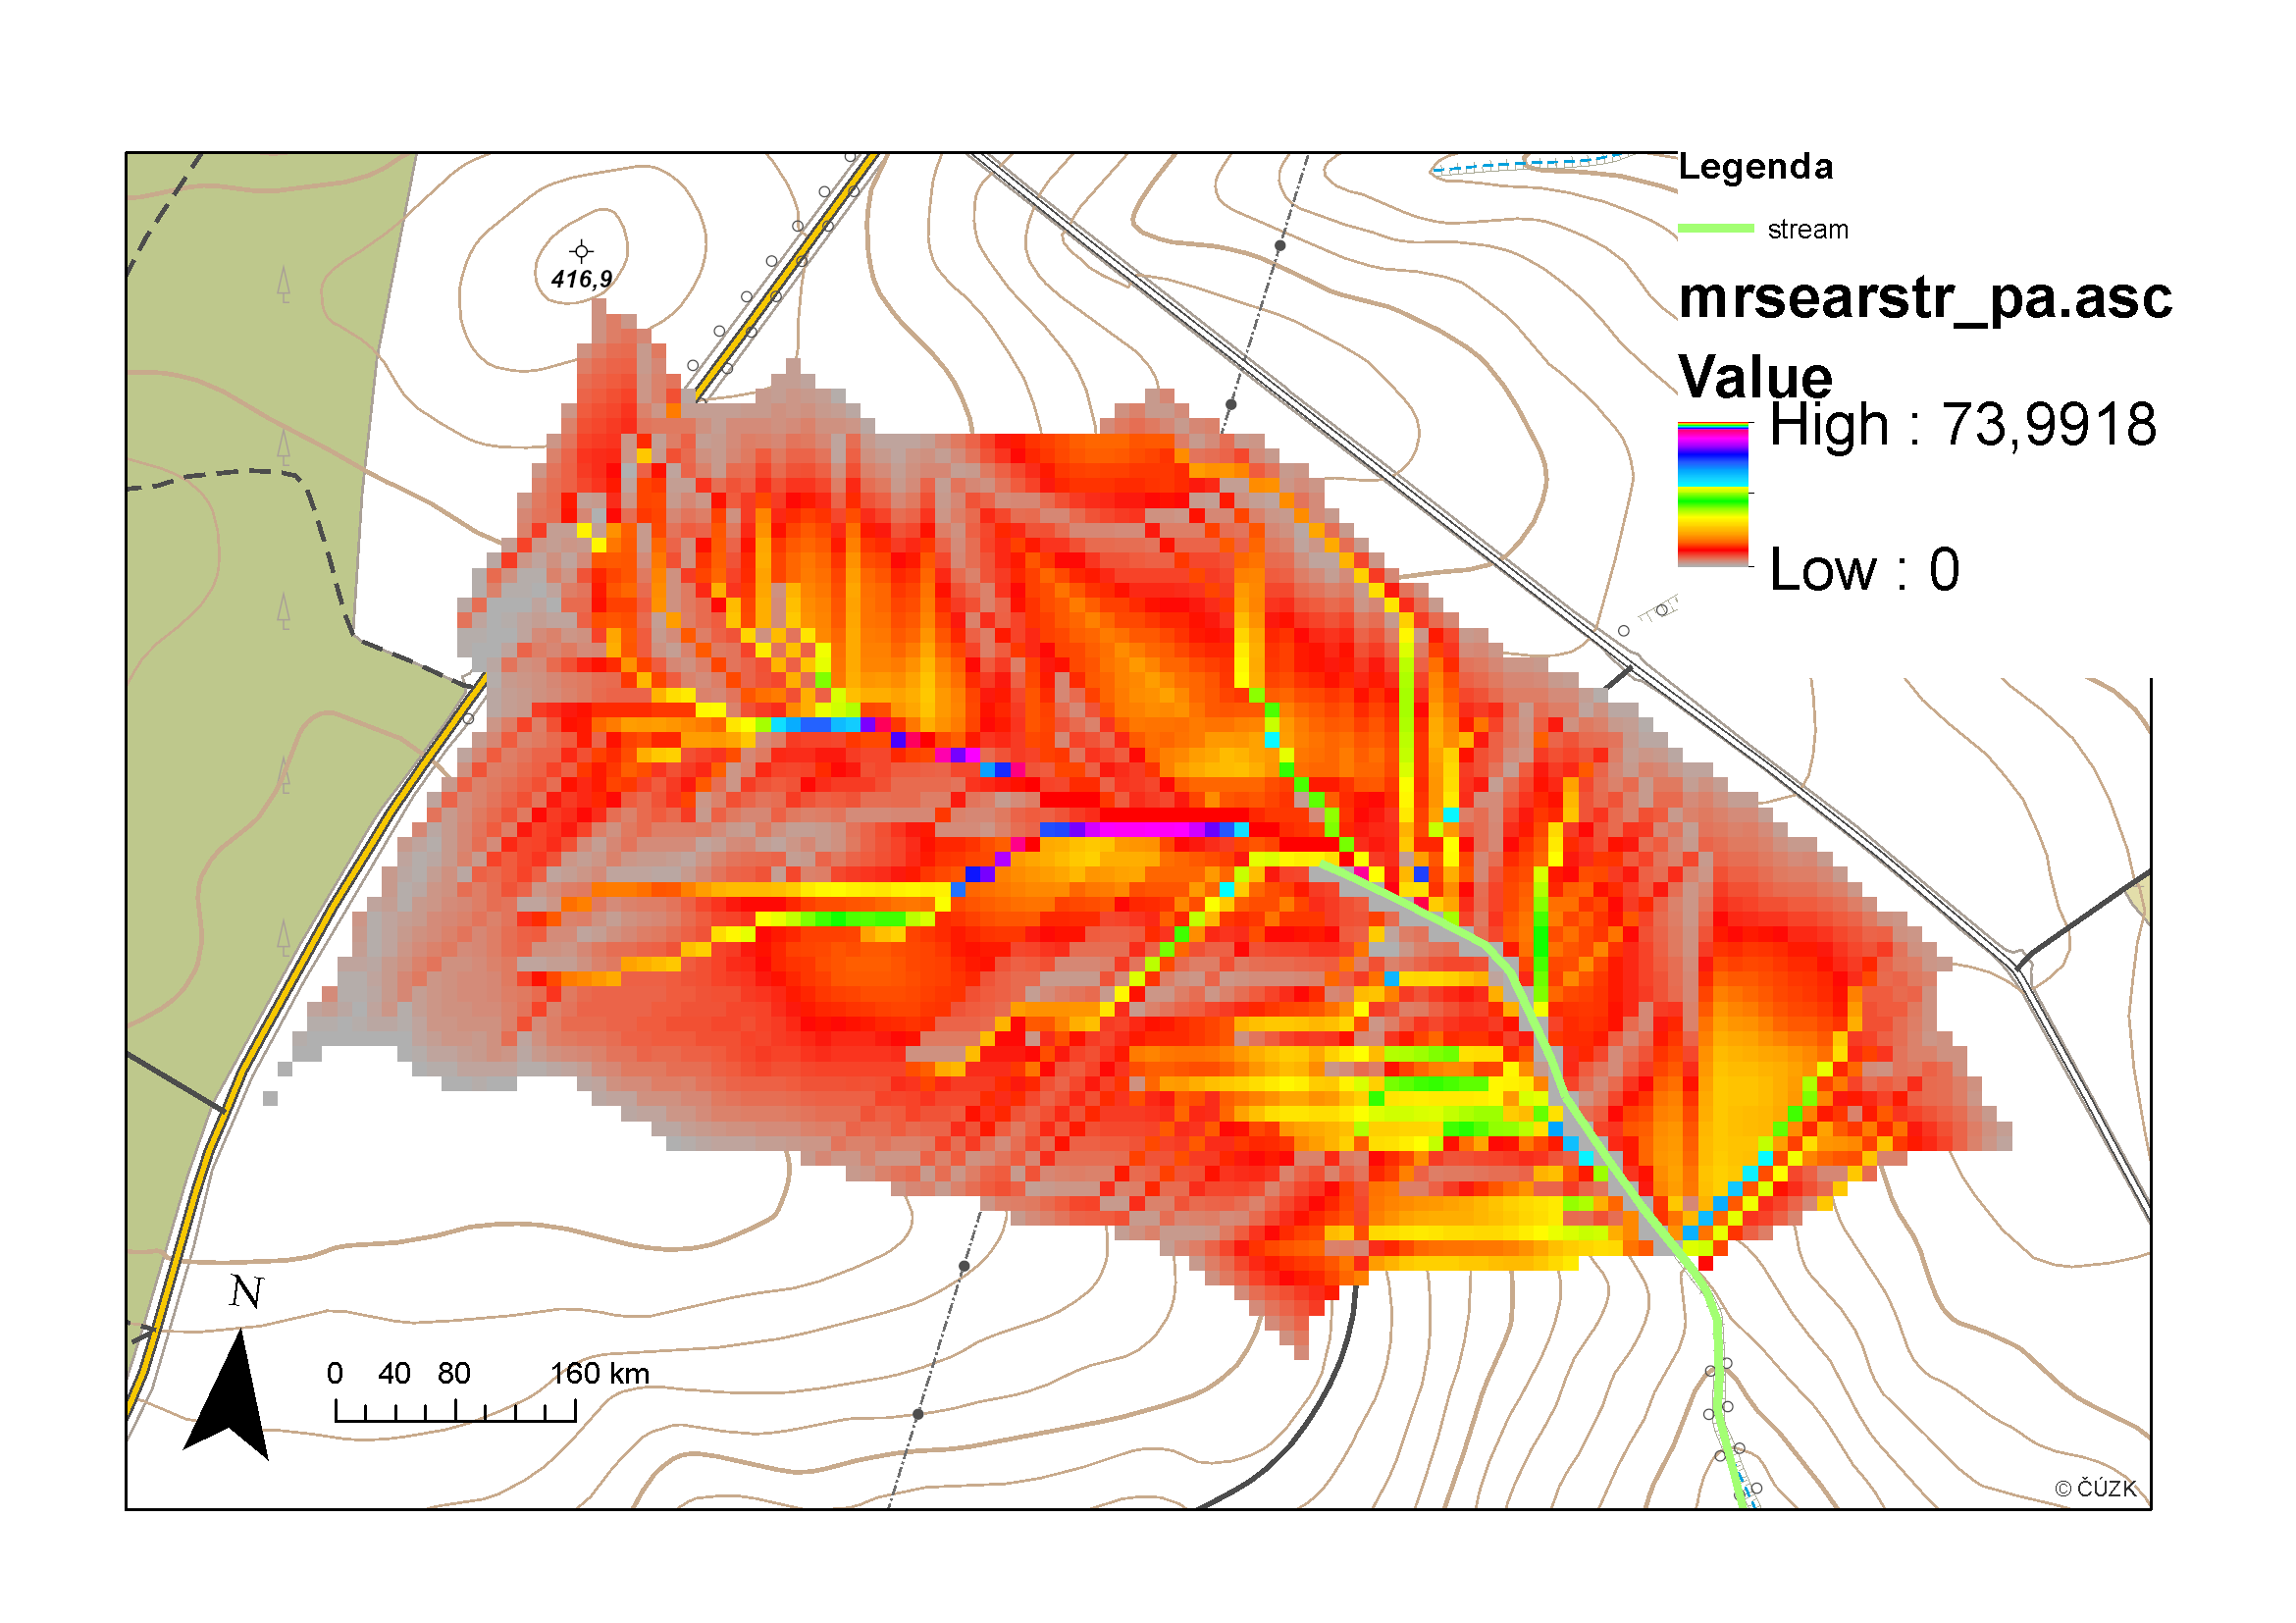
\includegraphics[width=0.55\textwidth]{obr/mshear.png}
            \end{adjustwidth}
        \end{frame}


        \begin{frame}[plain]
            Ukázka výsledků reakce povodí na 40 minut 120 mm/hod srážky
            %\begin{adjustwidth}{-4em}{-3em}
                %\begin{columns}
                    %\begin{column}{0.5\textwidth}
                    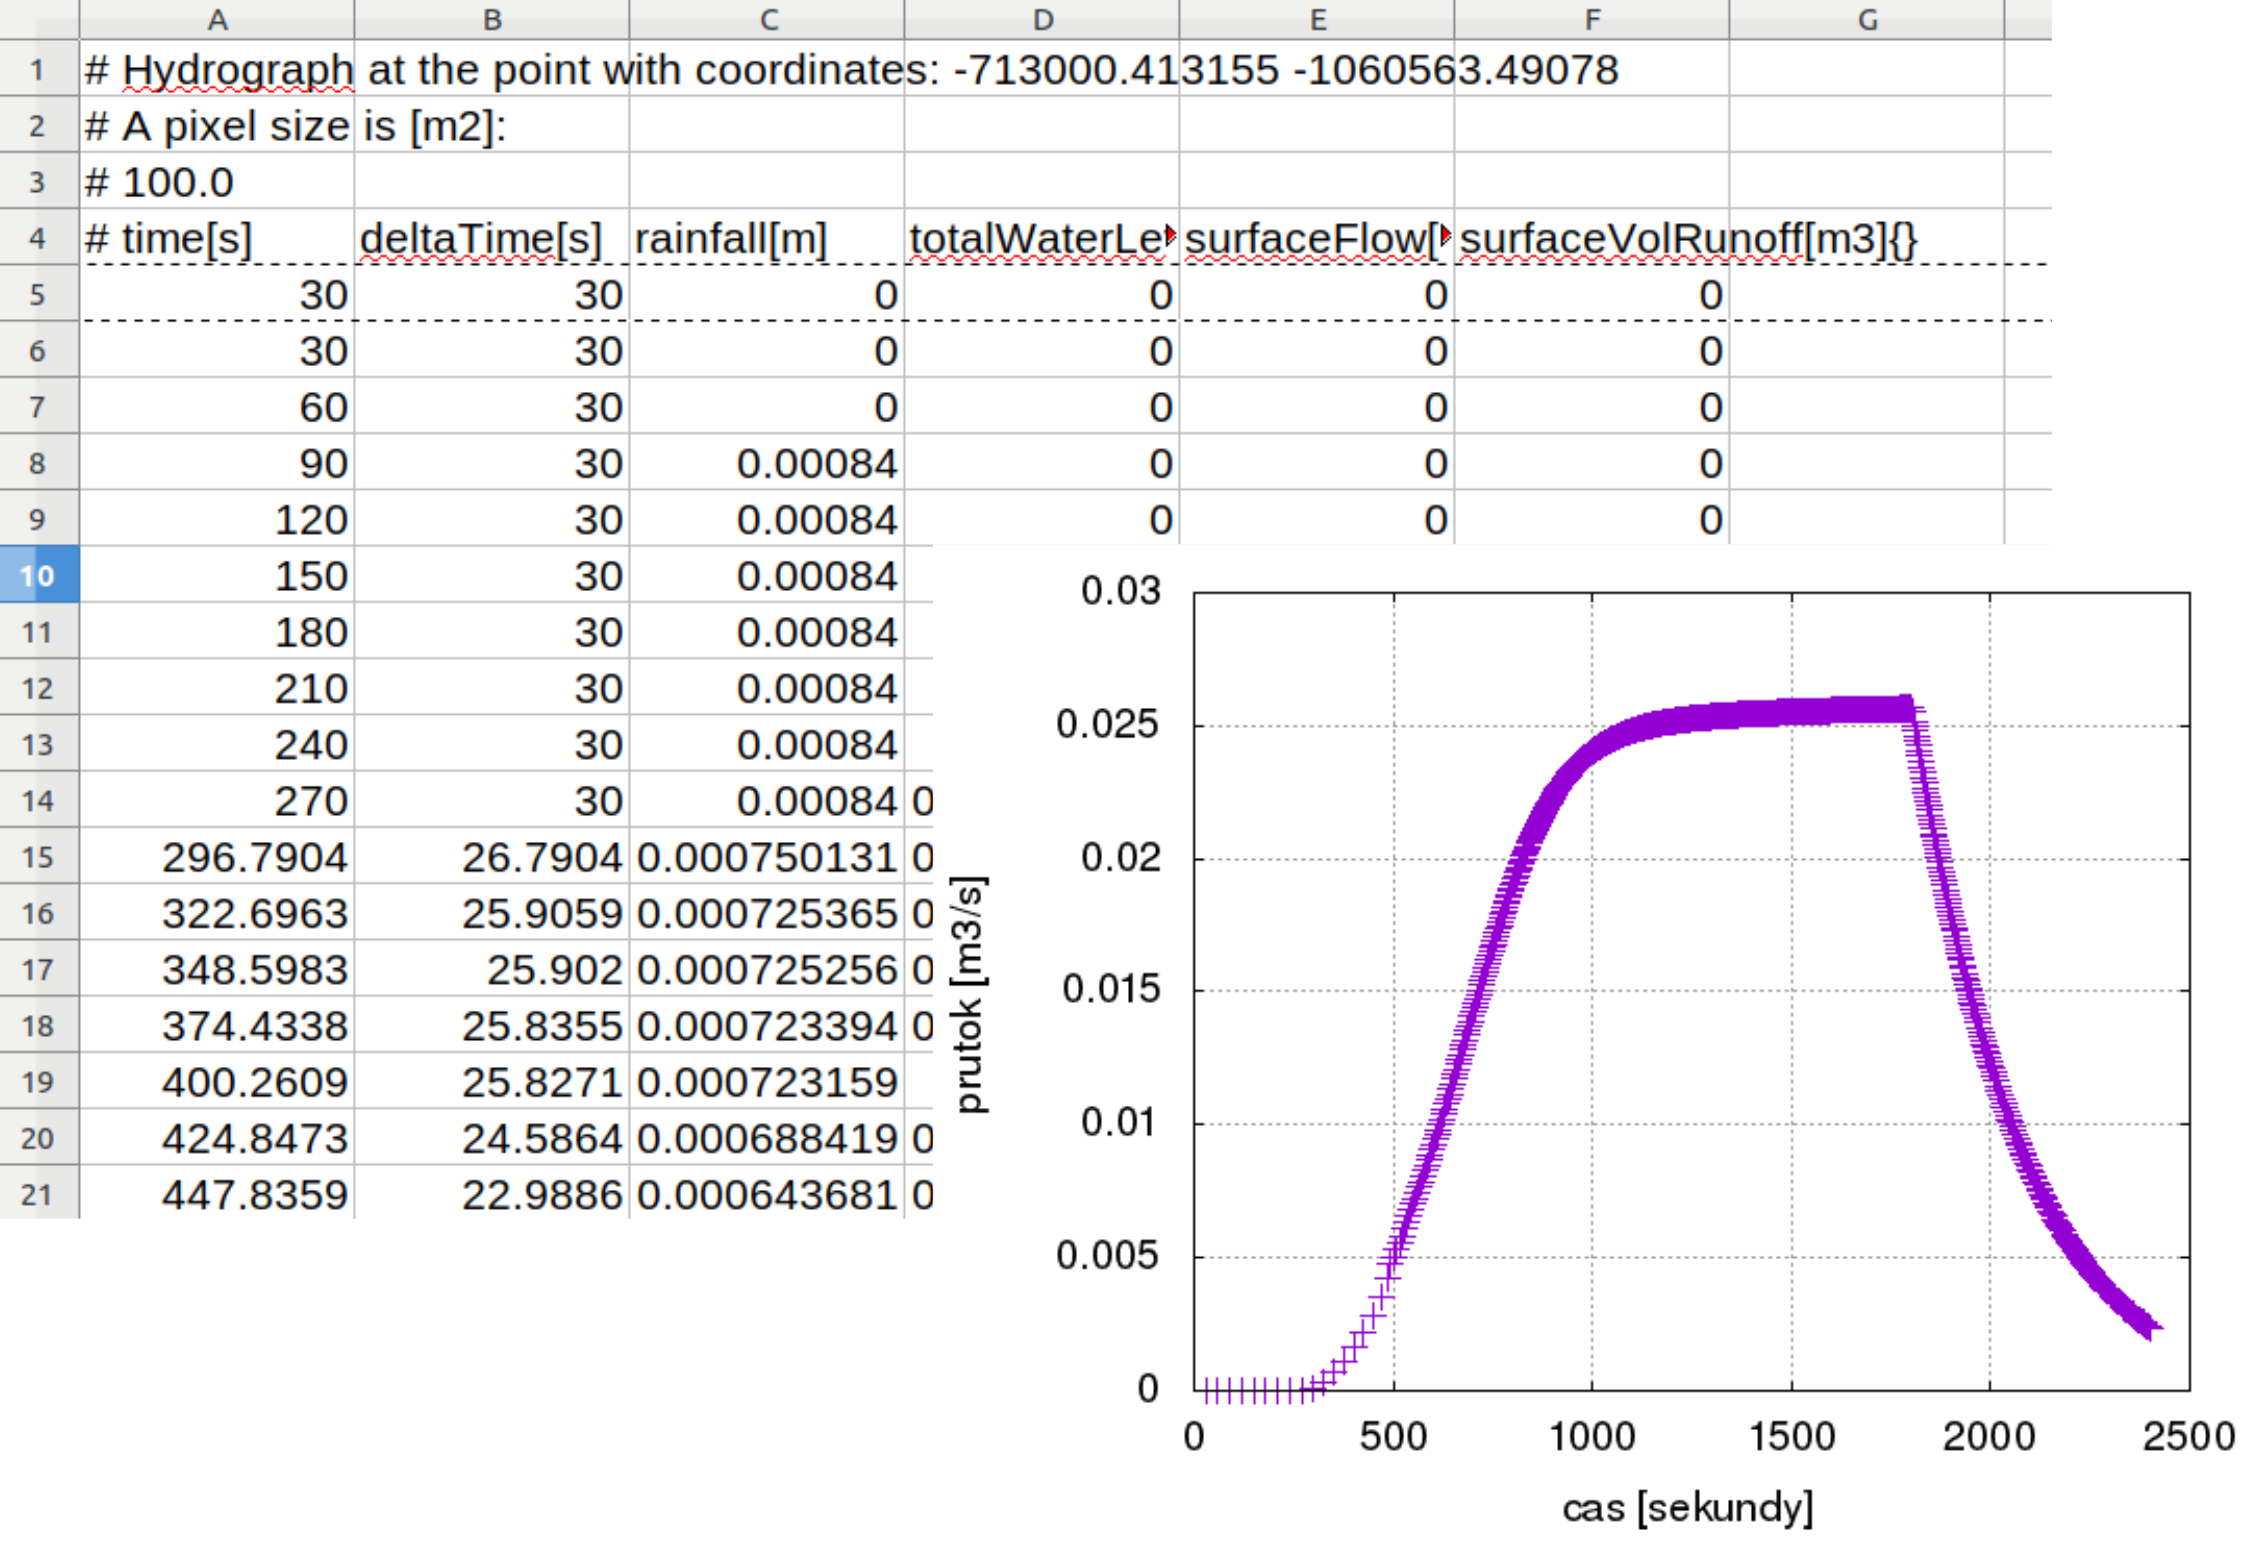
\includegraphics[width=0.9\textwidth]{obr/pointtab.png}
                    %\end{column}
                    %\begin{column}{0.5\textwidth}
                    %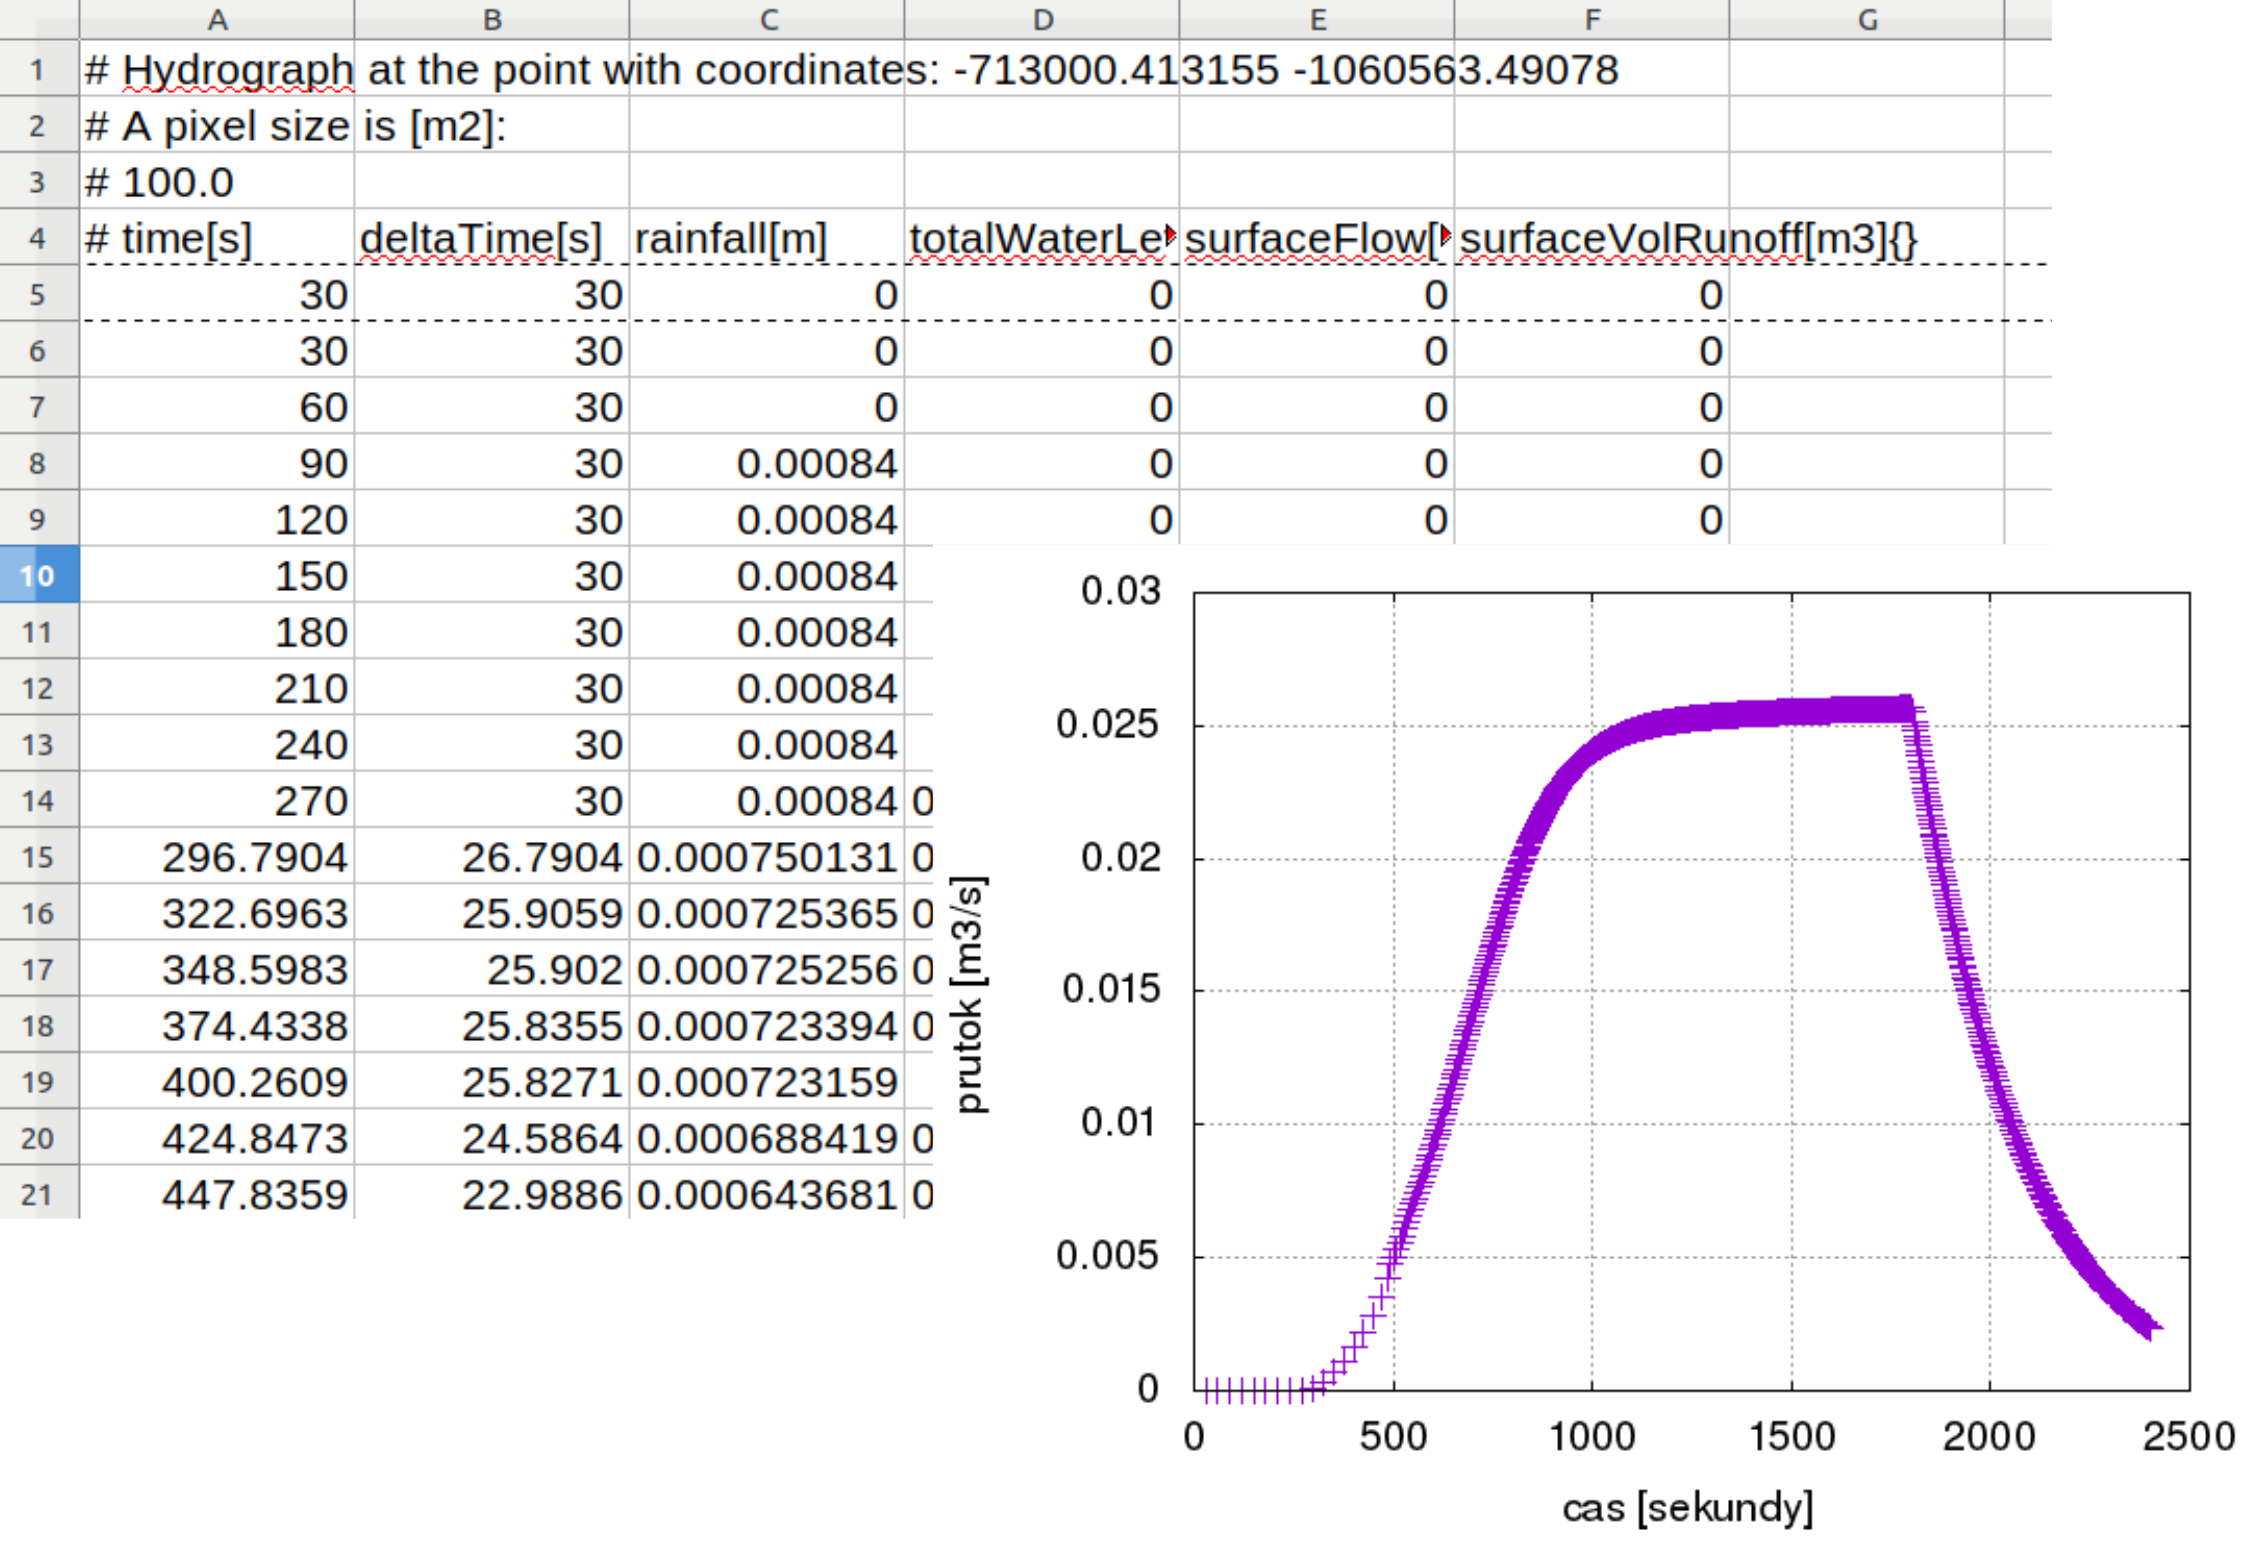
\includegraphics[width=1.1\textwidth]{obr/pointtab.png}
                    %\end{column}
                %\end{columns}
            %\end{adjustwidth}
        \end{frame}

    \section{Ke stažení}
\begin{frame}
    Stažení SMODERPU a další informace na: \href{http://storm.fsv.cvut.cz/cinnost-katedry/volne-stazitelne-vysledky/smoderp/?lang=cz}{storm.fsv.cvut.cz/../smoderp/}\vspace{1em}
    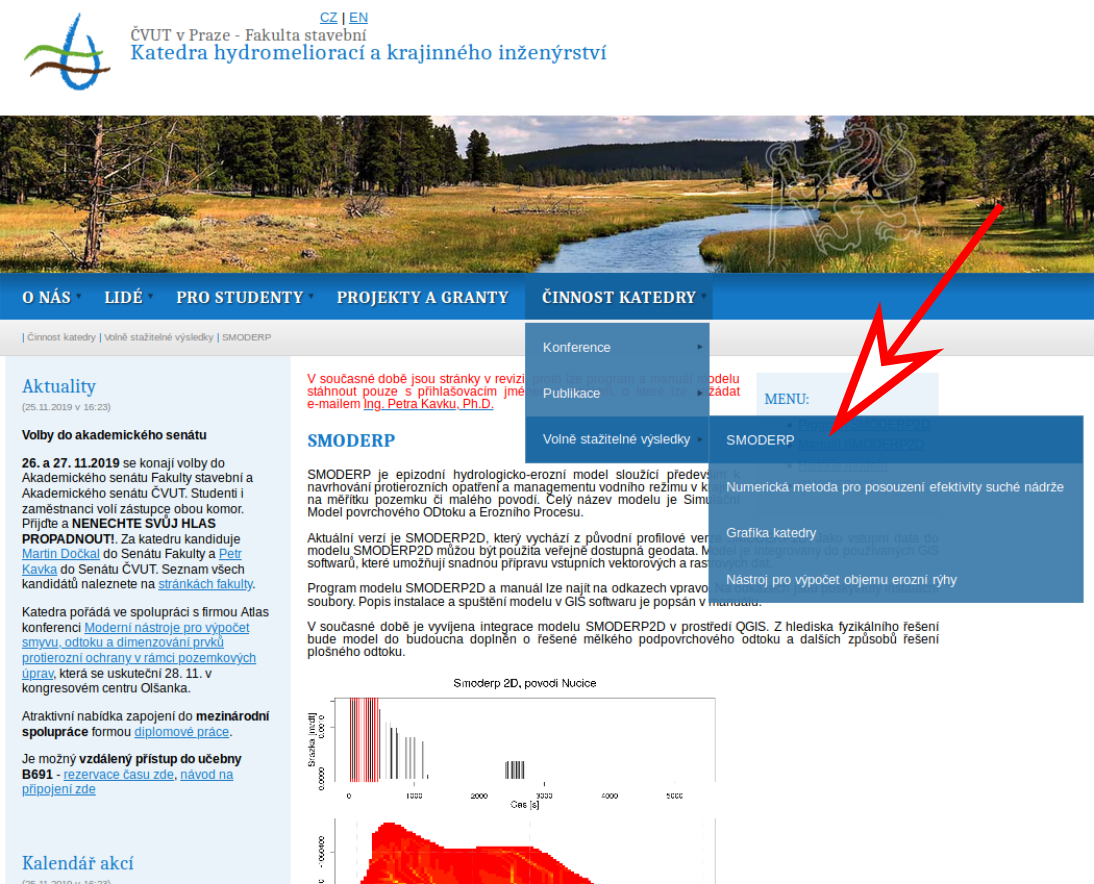
\includegraphics[height=0.9\textheight]{obr/storm-web.png}
\end{frame}
\begin{frame}
    Aktuální úpravy/opravy lze najít na github.com \href{https://github.com/storm-fsv-cvut/smoderp2d}{github.com/storm-fsv-cvut}\vspace{1em}
    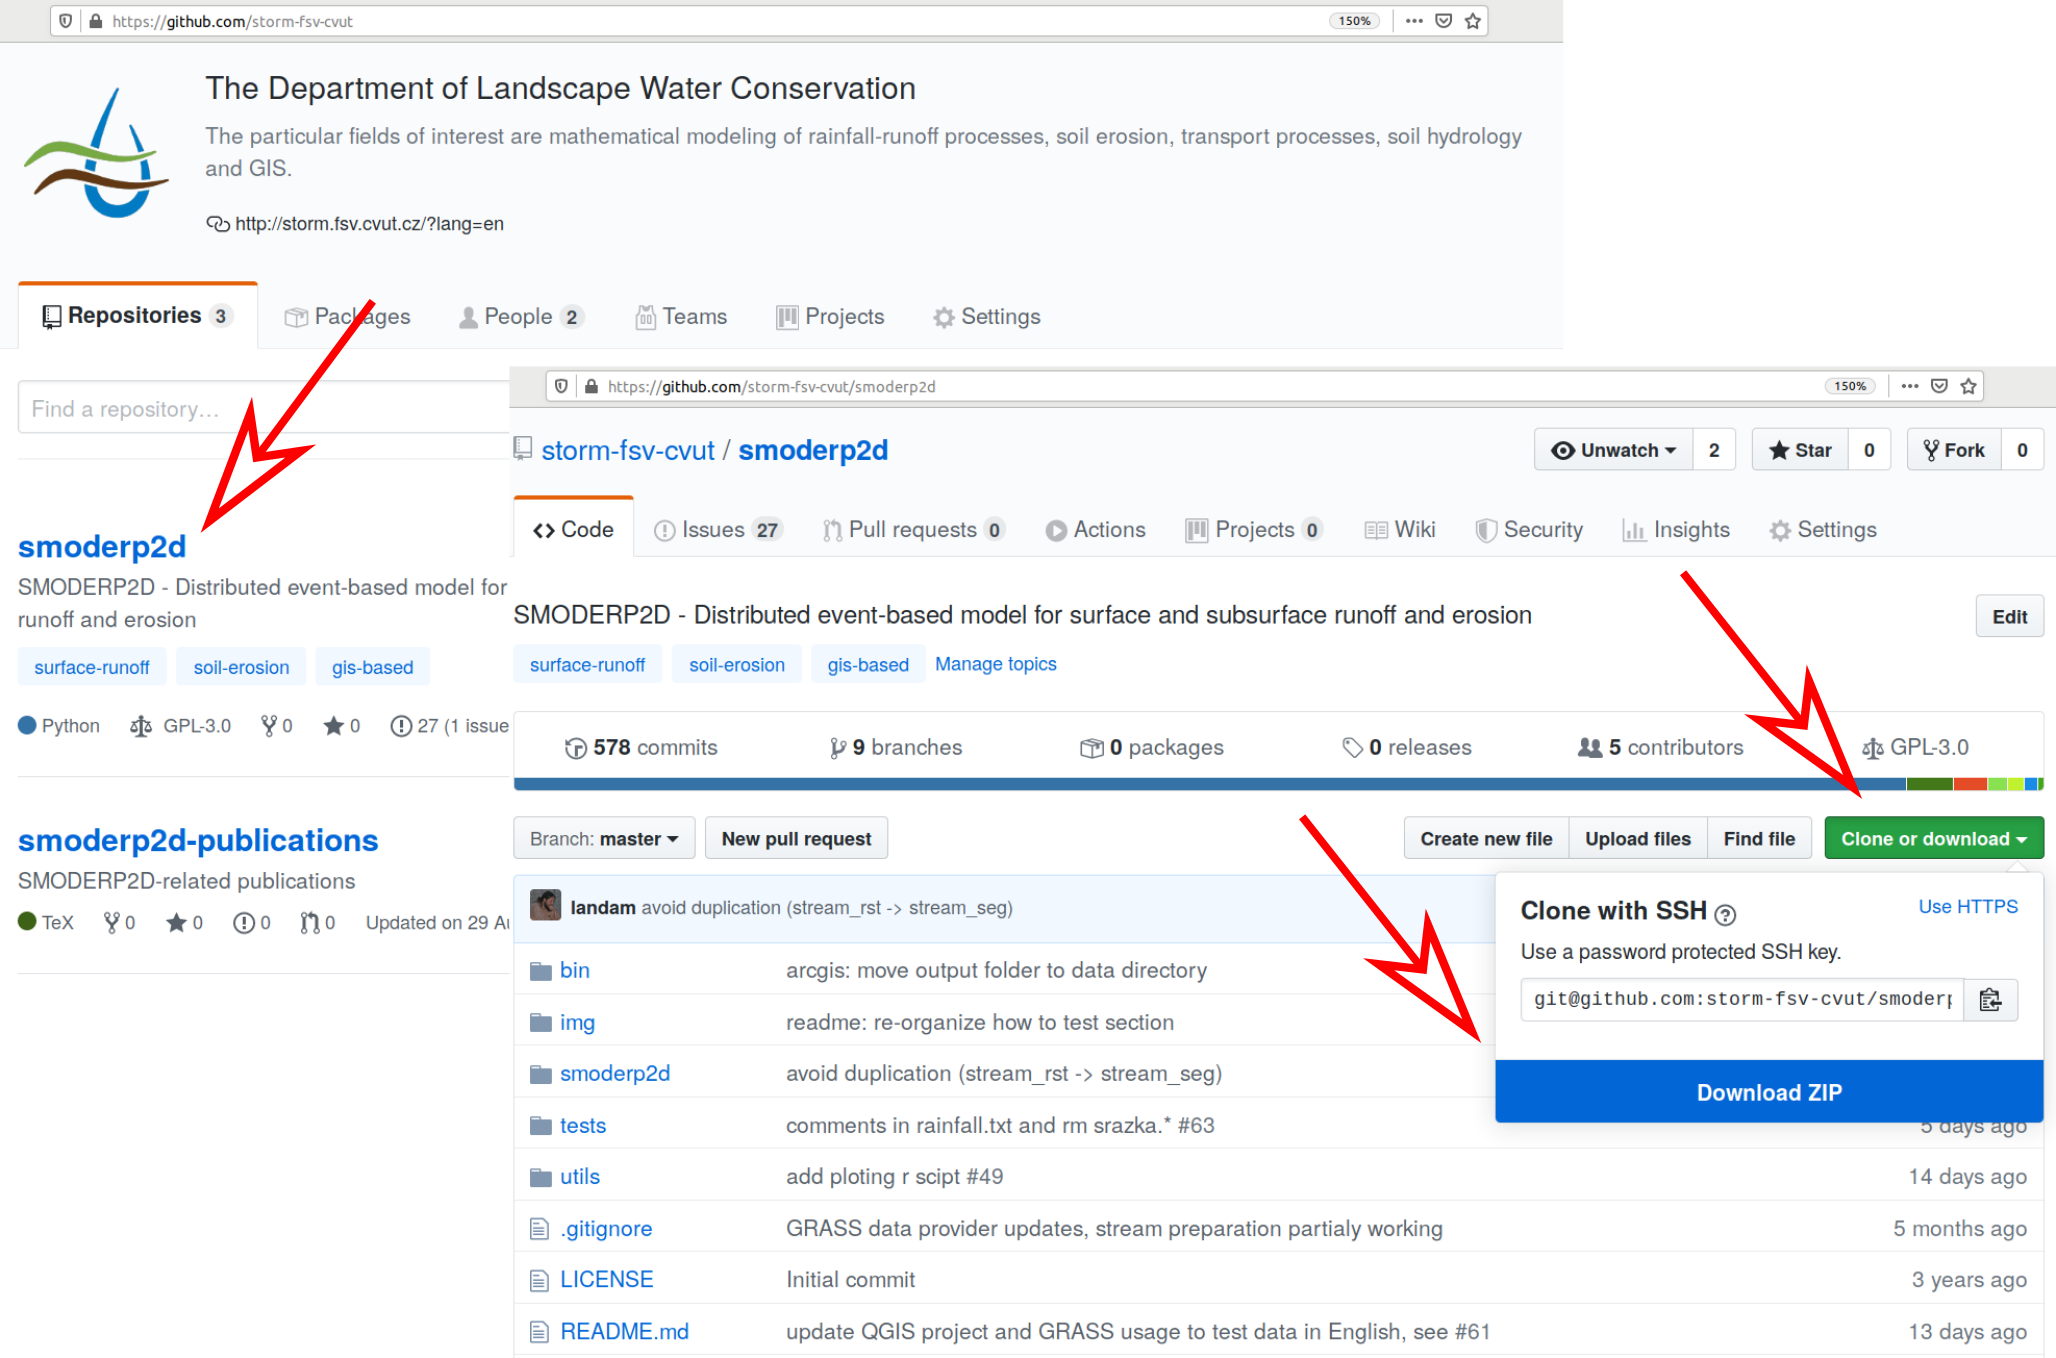
\includegraphics[width=\textwidth]{obr/git.png}
\end{frame}
\begin{frame}
    Testovací data v ArcGIS\vspace{1em}
    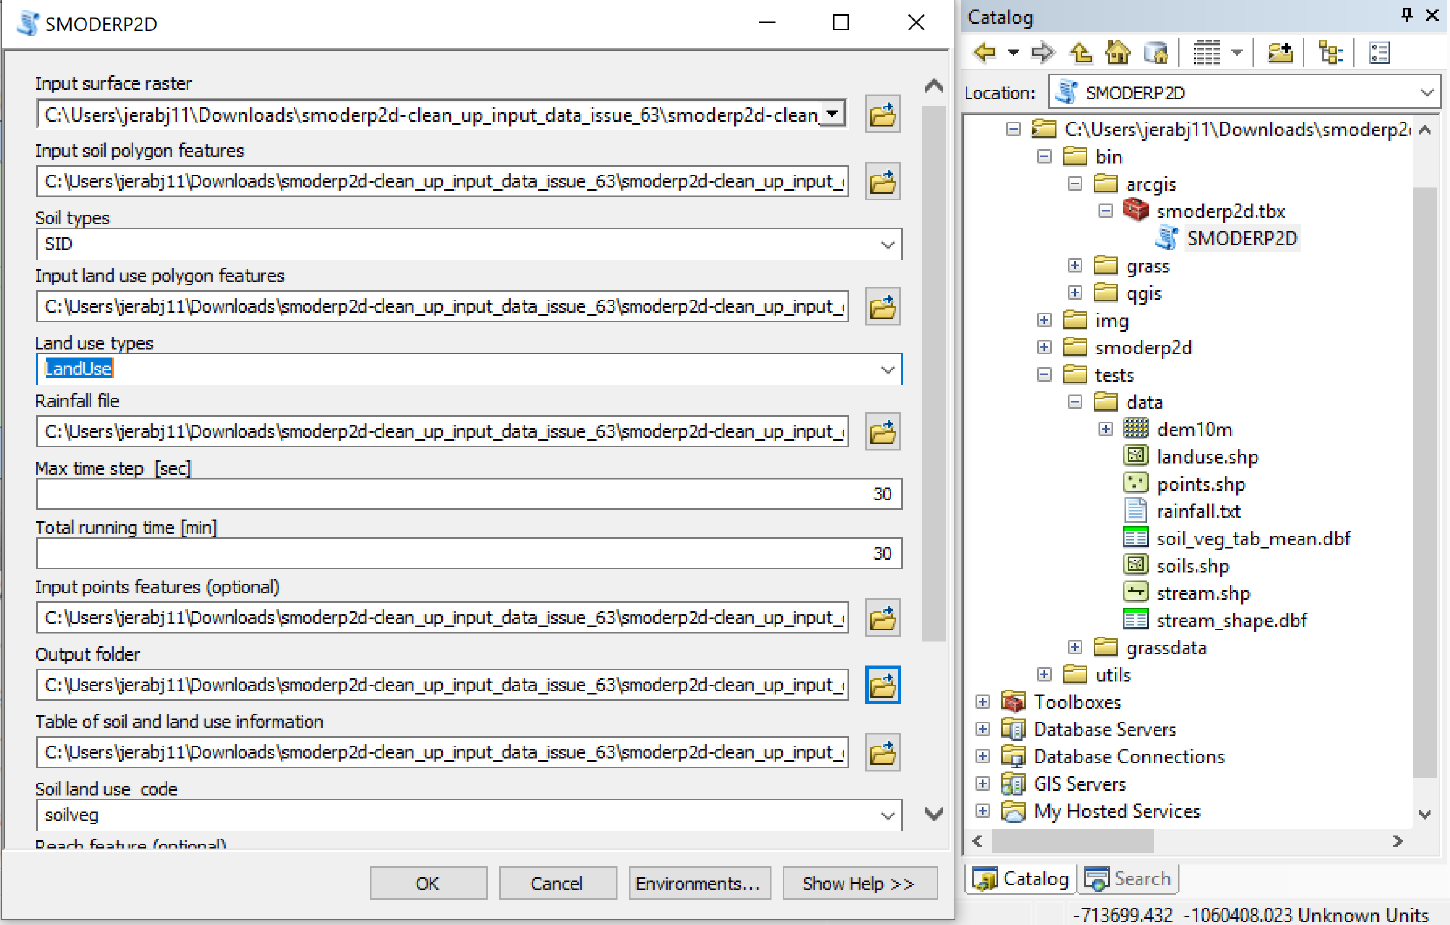
\includegraphics[width=0.95\textwidth]{obr/arcmap01.png}
\end{frame}

    \section{Závěr}
\begin{frame}
    Budoucnost:\vspace{1em}
    \begin{itemize}
        \item GRASS GIS, QGis (Q1, 2020)
        \item Vícesměrný odtok 
        \item Více infiltračních rutin
        \item Optimalizace numerického řešení
        \item Geoprocessingové služby\footnote{Landa:Geoprocessingové služby -moderní způsob vzdáleného zpracování prostorových dat}
    \end{itemize}
\end{frame}

% puvodni posledni slide
%\begin{frame}[plain]
    %
\includegraphics[height=0.175\textheight]{loga/logo_TACR_zakl.png}
    %\hfill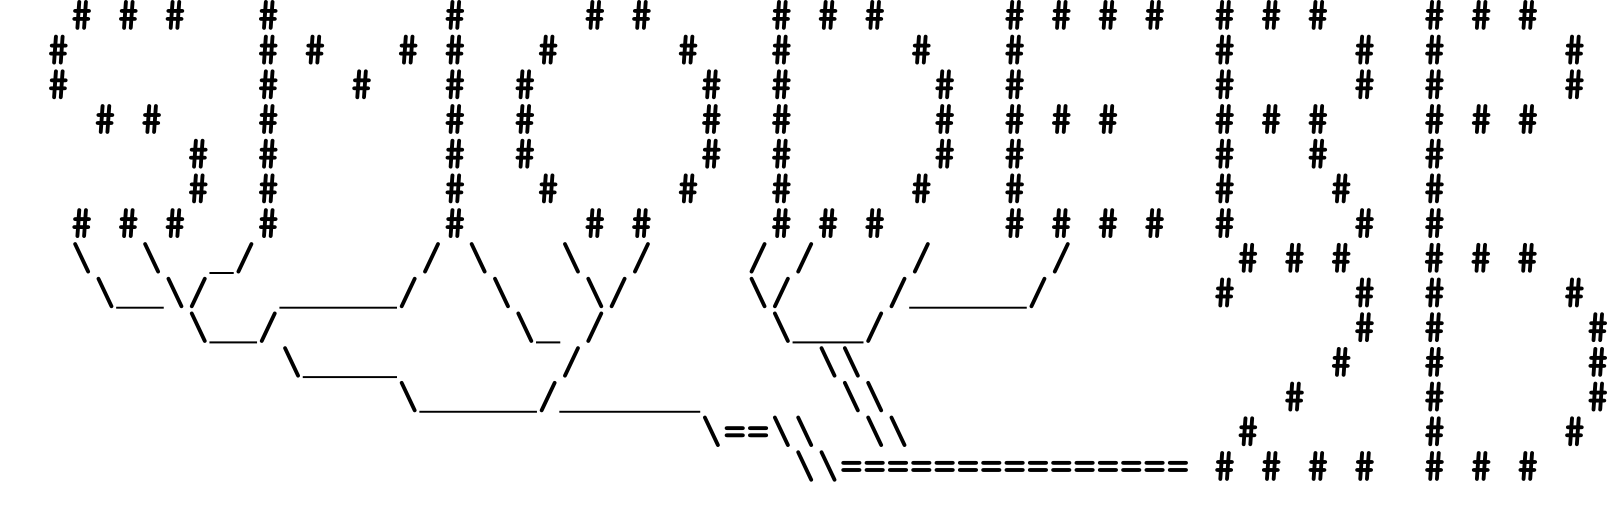
\includegraphics[height=0.175\textheight]{loga/logsmoderp.png}\\\vfill
    %
\includegraphics[height=0.175\textheight]{loga/logo_CVUT.jpg}
    %\hfill
\includegraphics[height=0.175\textheight]{loga/K143napisL_bar_3674x935.png}\\\vspace{1em}
    %\begin{center}{\Huge Děkuji za pozornost}\end{center}
%\end{frame}

\begin{frame}[plain]
    \begin{columns}
        \begin{column}{0.5\textwidth}
            \begin{itemize}
                \item Vyzkoušejte SMODERP2D
                \begin{itemize}
                    \item stránky katedry KHMKI \href{http://storm.fsv.cvut.cz/cinnost-katedry/volne-stazitelne-vysledky/smoderp/?lang=cz}{storm.fsv.cvut.cz/../smoderp/}
                    \item github.com \href{https://github.com/storm-fsv-cvut/smoderp2d}{github.com/storm-fsv-cvut}
                \end{itemize}
                \item Reportujte podněty
                \begin{itemize}
                    \item e-mailem: \href{mailto:petr.kavka@fsv.cvut.cz}{petr.kavka@fsv.cvut.cz} 
                    \item jako issue na github.com: \href{https://github.com/storm-fsv-cvut/smoderp2d/issues}{github.com/.../smoderp2d/issues}
                \end{itemize}
                \item Napište nám!
            \end{itemize}
        \end{column}
        \begin{column}{0.5\textwidth}
            \hfill
\includegraphics[height=0.15\textheight]{loga/logo_TACR_zakl.png}\\\vspace{0.5em}
            \hfill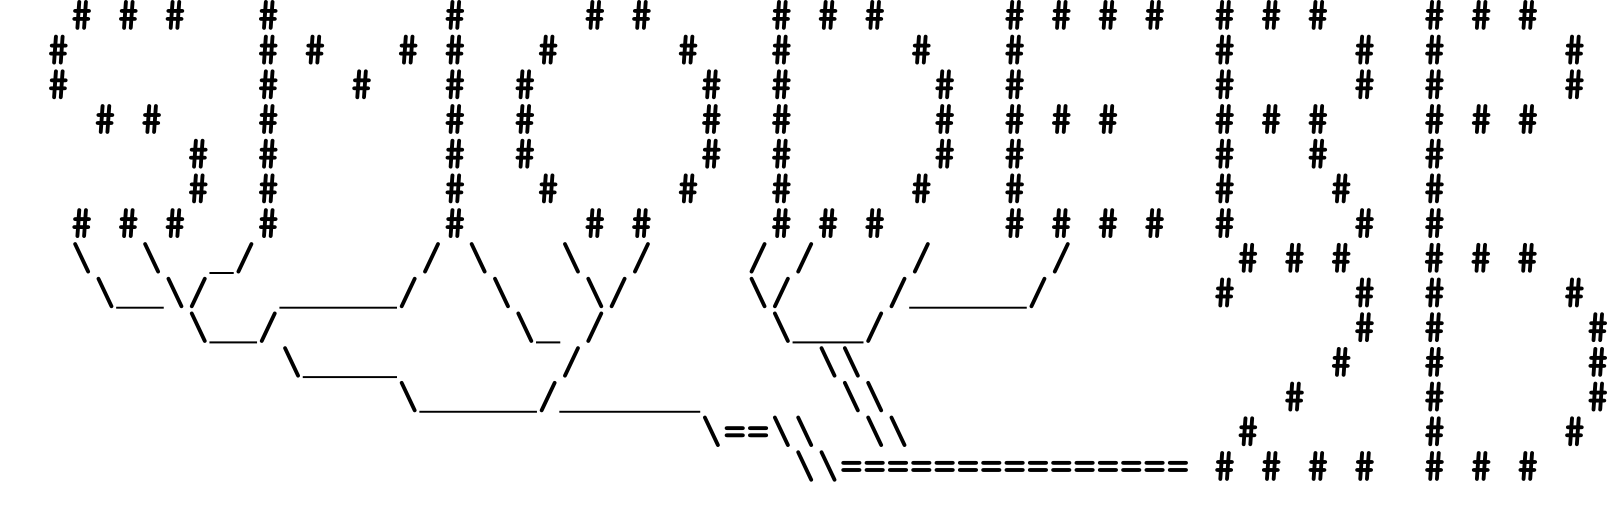
\includegraphics[height=0.15\textheight]{loga/logsmoderp.png}\\\vspace{0.5em}
            \hfill
\includegraphics[height=0.15\textheight]{loga/logo_CVUT.jpg}\\\vspace{0.5em}
            \hfill
\includegraphics[height=0.15\textheight]{loga/K143napisL_bar_3674x935.png}\\\vspace{0.5em}
        \end{column}
    \end{columns}
    \begin{center}{\Huge Děkuji za pozornost}\end{center}
\end{frame}


    \section{Appendix}
\begin{frame}
\begin{table}%[!htp]
  \centering
  \caption{Přehled parametrů charakterizujících půdní typ a typ vegetačního pokryvu}
  {\small
    \begin{tabular}{p{2cm}l}
    \hline  \hline
    Povinný název hlavičky v~tabulce & Popis \\
    \hline
        k&nasycená hydraulická vodivost [$m/s$] \\
        s&sorptivita [$s/m^{1/3}$] \\
        n&Manningův součinitel drsnosti [$mm$] \\
        pi&potenciální intercepce [$-$] \\
        ppl&poměrná plocha listová [$-$] \\
        ret&povrchová retence [$mm$] \\
        b&parameter plošného odtoku [$-$] \\
        x&parameter plošného odtoku [$-$] \\
        y&parameter plošného odtoku [$-$] \\
        tau&kritické tečné napětí[$Pa$]  \\
        v&kritická nevymílací rychlost [$m/s$] \\
    \hline  \hline
    \end{tabular}%
  }
  \label{tab:soilveg}%
\end{table}%

    \hyperlink{fig}{Zpět}
\end{frame}


\end{document} 


